\documentclass{report}

% ----------------------------------------------------------------------------
% Preamble
% ----------------------------------------------------------------------------

% These are some lazy packages to get a good looking page layout
\usepackage{fullpage}
\usepackage[parfill]{parskip}
\usepackage[toc,page]{appendix}

\usepackage{setspace}
\onehalfspacing

% A package to include graphics files (jpg, png, eps, pdf etc...)
%\usepackage{epstopdf}
\usepackage{graphicx}
\usepackage{caption}
\usepackage{subcaption}
\usepackage{color}

% Some basic packages that are almost standad
\usepackage{amssymb}
\usepackage{amsmath}
\usepackage{amsthm}

% Package to be able to draw tikz images
\usepackage{tikz}
\usetikzlibrary{calc}
\usetikzlibrary{decorations.pathreplacing}

% Package to get hyperrlinks
\usepackage{hyperref}

% Package to be able to compile standalone tikz packages
\usepackage{standalone}

% Notes
\usepackage{todonotes}

% Code
\usepackage{listings}

% A package that gives more control for bibliographies than the default
\usepackage[backend=biber, backref=true, firstinits=true, url=true, isbn=true]{biblatex}
\addbibresource{bibliography.bib}

% ----------------------------------------------------------------------------
% Some useful definitions
% ----------------------------------------------------------------------------

\renewcommand{\v}[1]{\mathbf{#1}}
\newcommand{\generalLaplaceEqn}{-\nabla\cdot(a\nabla{u}) + \v{b}\cdot\nabla{u} + cu &= f}
\newcommand{\half}{\frac{1}{2}}
\newcommand{\myref}[1]{(\ref{#1})}
\newcommand{\incode}[1]{\framebox{\textit{#1}}}

% ----------------------------------------------------------------------------
% Code listing settings
% ----------------------------------------------------------------------------
\definecolor{commentgreen}{rgb}{0.0, 0.6, 0.0}

\lstset{ %
    backgroundcolor=\color{white},
    basicstyle=\footnotesize,
    breakatwhitespace=true,
    breaklines=true,
    captionpos=b,
    commentstyle=\color{commentgreen},
    frame=trBL,
    frameround=fttt,
    keepspaces=true,
    numbers=left,
    showspaces=false,
    tabsize=2,
    title=\lstname
}

% ----------------------------------------------------------------------------
% The actual report
% ----------------------------------------------------------------------------

\begin{document}
    \begin{titlepage}
    \begin{center}
        \vspace*{5cm}

        \textbf{Polynomial Chaos}

        \vspace{0.5cm}
        Thesis Subtitle

        \vspace{1.5cm}

        \textbf{Alex Carney}

        \vfill

        MMath. Final Year Dissertation\\

        \vspace{0.5cm}
        Cardiff School of Mathematics

        \vspace{1.5cm}

        
\includegraphics[width=0.4\textwidth]{../img/universitylogo.eps}


    \end{center}
\end{titlepage}

    \Huge{\textbf{Acknowledgments}}

\normalsize

\vspace{1.5cm}



    \listoftodos

    \tableofcontents
    \listoffigures

    % The actual content:
    \chapter{One Dimensional Deterministic Case}\label{chap:oned-deterministic}

\todo[inline]{Change domain notation}

The simplest form of Laplace's Equation we can consider is the one dimensional
case where the coefficients are deterministic in which case the equation is
given by:

\begin{equation}\label{eq:oned-deterministic}
\begin{aligned}
    -au''(x) + bu'(x) + cu(x) &= f(x) &\text{ in } \Omega = [0, 1] \\
                         u(x) &= 0 &\text{ on } \delta\Omega = \{0, 1\}
\end{aligned}
\end{equation}

We consider the equation in the interval $[0,1]$ and prescribe a zero Dirichlet
condition at the endpoints $x = 0$ and $x = 1$.

\todo[inline]{In the deterministic case, we should be able to solve various
versions of this analytically. Include a few such cases and their solutions
they will provide us with a few good examples to compare our numerical
solutions with}

\section{Weak Formulation}

\todo[inline]{Give proper definitions of $V$ and $W$}
\todo[inline]{Justify the necessity of the weak formulation}

The first step in implementing the finite element method is to obtain the weak
formulation of this problem. To get the continuous weak form of the equation,
we multiply through by $v \in W$ and integrate over the domain:

\begin{equation}
    -a\int_0^1{u''(x)v(x)\ dx} + b\int_0^1{u'(x)v(x)\ dx}
    + c\int_0^1{u(x)v(x)\ dx} = \int_0^1{f(x)v(x)\ dx}
\end{equation}

Integrating the first term by parts gives us:

\begin{equation}
    -a\int_0^1{u''(x)v(x)\ dx} = -a\underbrace{[ u'(x)v(x) ]_0^1}_{ = 0}
    + a\int_0^1{u'(x)v'(x)\ dx}
\end{equation}

Where the underbraced term is zero as $v$ is zero at the endpoints of the
domain. Hence the continuous weak form of \myref{eq:oned-deterministic} is given
by:

\begin{equation}\label{eq:wk-oned-deterministic}
    a\int_0^1{u'(x)v'(x)\ dx} + b\int_0^1{u'(x)v(x)\ dx}
    + c\int_0^1{u(x)v(x)\ dx} = \int_0^1{f(x)v(x)\ dx}
\end{equation}

And a weak solution would be to find $u \in V$ such that, the above equation is
satisfied $\forall v \in W$

\section{Discrete Formulation}

\begin{figure}
\centering
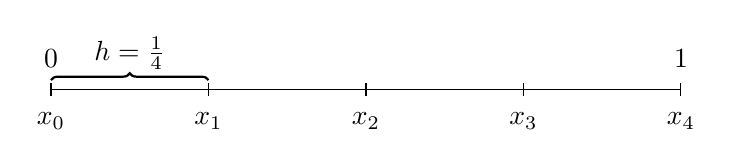
\begin{tikzpicture}[scale=8]
    % Draw the 0-1 interval
    \draw (0,0) -- (1, 0);

    % Draw the 'ticks' along the axis as well as the labels
    \foreach \x in {0,...,4}
    {
        \draw (0.25*\x, 0.01) -- (0.25*\x, -0.01);
        \node (\x) at (0.25*\x, -0.05) {$x_\x$};
    }

    % Draw the 0, 1 labels
    \node () at (0, 0.05) {0};
    \node () at (1, 0.05) {1};

    % Finally demonstrate the length of the interval
    \draw[thick, decoration={brace}, decorate] (0, 0.015) -- (0.25, 0.015)
        node[pos=0.5, anchor=south] {$h = \frac{1}{4}$};
\end{tikzpicture}


\caption{Example discretisation with N = 4}
\label{fig:one-d-discretisation}
\end{figure}

For a given parameter $N \in \mathbb{N}$ we define $N+1$ equally spaced nodes
$x_i$ $i \in \{0, \ldots, N\}$ in the interval $[0,1]$ where
$x_0 = 0, x_N = 1$. Then we can divide the domain into $N$ subintervals
$ I_i = [x_i, x_{i+1}]$, $i \in \{0,\ldots,N - 1\}$ of length $h = \frac{1}{N}$.
We can then define our discretisation to be:

\[
    D^h = \bigcup_{i=0}^{N - 1} I_i
\]

See Figure \ref{fig:one-d-discretisation} for an example discretisation
when $N=4$.  Upon such a discretisation we can define suitable finite
dimensional subspaces of our trial and test spaces $V^h \subset V$, $W^h
\subset W$.

\begin{align*}
    V^h &= \{v \in V: v \text{ is linear on } I_i,
          \ i \in \{0, \ldots, N - 1\},
          v \text{ is continuous on } [0, 1]\} \\
    W^h &= \{w \in W: w \text{ is linear on } I_i,
          \ i \in \{0, \ldots, N - 1\},
          w \text{ is continuous on } [0, 1]\}
\end{align*}

By choosing appropriate basis functions $\phi_i$ that span the space, we will
be able to approximate the solution as such:

\begin{equation}\label{eq:one-d-approx-soln}
    u^h(x) = \sum_{j = 0}^N{u_j\phi_j(x)}
\end{equation}

where $u_i$ will be the approximate value of the solution at the node $x_i$. In
a similar manner we will also be able to approximate $f(x)$:

\begin{equation}
    f(x) \approx \sum_{j = 0}^N f_j\phi_j(x)
\end{equation}

where $f_i = f(x_i)$. By writing the functions $u$ and $f$ in terms of their
values at the nodes $x_i$ then by taking a sufficiently large number of nodes
we can approximate them to within an acceptable margin of error.

\todo[inline]{Give an estimate for the error of the FEM for this problem -
Use the book!!}
\todo[inline]{Possibly include mention of existence and uniqueness of the
solution - Use the book !!}

An appropriate basis would be the so called `hat functions' which we can define
for each interior node as follows:

\begin{equation}\label{eq:one-d-hat-basis}
    \phi_i(x) = \left\{\begin{array}{c c}
                    \frac{x - x_{i-1}}{x_i - x_{i - 1}}, & x \in [x_{i-1}, x_i] \\
                    \frac{x_{i+1} - x}{x_{i + 1} - x_i}, & x \in [x_i, x_{i + 1}] \\
                    0, & \text{otherwise}
                \end{array}\right.
\end{equation}

And in the special case of the boundary nodes $x_0$ and $x_N$ we only consider
the intervals which lie in our domain:

\begin{align}
    \phi_0(x) &= \left\{\begin{array}{c c}
                    \frac{x_1 - x}{x_1 - x_0}, & x \in [x_0, x_1] \\
                    0, & \text{otherwise}
    \end{array}\right.
    \\
    \phi_N(x) &= \left\{\begin{array}{c c}
                    \frac{x - x_{N - 1}}{x_N - x_{N-1}}, & x \in [x_{N-1}, x_N] \\
                    0, & \text{otherwise}
    \end{array}\right.
\end{align}

As the weak formulation \myref{eq:wk-oned-deterministic} must be satisfied for
all $v \in W$ then in particular it must be satisfied for the basis functions
$\phi_i(x)$. So by taking $v = \phi_i(x)$ for each $i \in \{1,\ldots,N\}$ and
substituting our approximations for $u$ and $f$ we obtain:

\begin{align*}
    a\int_0^1{\left(\sum_{j = 0}^N{u_j\phi_j(x)}\right)'\phi_i'(x)\, dx}
    &+b\int_0^1{\left(\sum_{j = 0}^N{u_j\phi_j(x)}\right)'\phi_i(x)\, dx} \\
    &+c\int_0^1{\left(\sum_{j = 0}^N{u_j\phi_j(x)}\right)\phi_i(x)\, dx} =
    \int_0^1{\left(\sum_{j = 0}^Nf_j\phi_j(x)\right)\phi_i(x)\, dx}
\end{align*}

By the linearity of the integrals and derivatives we can write this as:

\begin{align*}
    a\sum_{j = 0}^Nu_j\int_0^1\phi_i'(x)\phi_j'(x)\, dx
    &+b\sum_{j = 0}^Nu_j\int_0^1\phi_i(x)\phi_j'(x)\, dx \\
    &+c\sum_{j = 0}^Nu_j\int_0^1\phi_i(x)\phi_j(x)\, dx =
    \sum_{j = 0}^Nf_j\int_0^1\phi_i(x)\phi_j(x)\, dx
\end{align*}

for each $i \in \{1,\ldots,N\}$. Or equivalently:

\begin{align}\label{eq:oned-deterministic-discrete}
  \begin{split}
    \sum_{j = 0}^N\underbrace{\left(a\int_0^1\phi_i'(x)\phi_j'(x)\, dx
        + b\int_0^1\phi_i(x)\phi_j'(x)\, dx + c\int_0^1\phi_i(x)\phi_j(x)\, dx\right)}_{:= A_{i,j}}u_j  \\
    = \sum_{j = 0}^N\underbrace{\int_0^1{\phi_i(x)\phi_j(x)}\, dx}_{:= M_{i,j}}f_j
  \end{split}
\end{align}

This effectively reduces the weak formulation \myref{eq:wk-oned-deterministic}
to a linear system $Au^h = Mf$ where $A$ is known as the stiffness matrix and
$M$ is known as the mass matrix. Being a linear system it is relatively
straightforward to solve solve computationally for the unknown vector $u^h$ and
by taking a sufficiently fine discretisation we can achieve a good
approximation to the actual solution $u$.

\begin{equation}
    \sum_{j=0}^NA_{i,j}u_i = \sum_{j=0}^NM_{i,j}f_i,\ i \in \{0,\ldots,N\}
\end{equation}

However due to the Dirichlet condition we have in \myref{eq:oned-deterministic}
we already know the value of $u$ at the nodes $x_0$ and $x_N$ so in the cases
where $j = 0$ and $j = N$ the associated terms on the left hand side can be
removed from the system of equations. Furthermore as we knows the value of our
solution $u$ at these nodes, we can move the associated terms over to the right
hand side:

\begin{equation}
    \sum_{j=1}^{N-1}A_{i,j}u_i =
        \sum_{j=1}^{N}M_{i,j}f_j - A_{i,0}u(0) - A_{i,N}u(1)
\end{equation}

In our particular problem we have a zero Dirichlet condition so the linear
system reduces quite nicely to:

\begin{equation}\label{eq:oned-deterministic-fem}
    \sum_{i=1}^{N-1}\sum_{j=1}^{N-1}A_{i,j}u_j
        = \sum_{i=1}^{N-1}\sum_{j=0}^NM_{i,j}f_j,\ i \in \{1,\dots,N-1\}
\end{equation}

Solving this system for the vector $\v{u}$ will give us the approximate
solution to the equation \myref{eq:oned-deterministic}

\section{Constructing the Global Linear System}

The final step in implementing the finite element method is to assemble the
global system of equations i.e.  determining the entries of $A_{i,j}$ and
$M_{i,j}$ which we currently have written in terms of a number of integrals
\myref{eq:oned-deterministic-discrete}. Due to the fact that our domain has
been subdivided into many subintervals we can consider the contribution from
each and combine them later into the global system.

\begin{figure}
\centering
\begin{tikzpicture}[scale=6]

    % Draw the axis
    \draw[thin] (-1.25, 0) -- (1.25, 0);

    % Draw the endpoints
    \draw (-1.25, 0.02) -- (-1.25, -0.02);
    \draw (1.25, 0.02) -- (1.25, -0.02);
    \node (0) at (-1.25, -0.07) {$x_0$};
    \node (N) at (1.25, -0.07) {$x_N$};

    % Draw the dot dot dots
    \node (1) at (-1, -0.07) {$\cdots$};
    \node (2) at (1, -0.07) {$\cdots$};

    % Draw the supporting nodes
    \draw (-0.75, 0.02) -- (-0.75, -0.02);
    \draw (0.75, 0.02) -- (0.75, -0.02);
    \node (k0) at (-0.75, -0.07) {$x_{k-1}$};
    \node (k3) at (0.75, -0.07) {$x_{k+2}$};

    % Draw the intervals we are interested in
    \draw (-0.25, 0.02) -- (-0.25, -0.02);
    \draw (0.25, 0.02) -- (0.25, -0.02);
    \draw[dotted] (-0.25, 0) -- (-0.25, 0.5);
    \draw[dotted] (0.25, 0) -- (0.25, 0.5);
    \node (k1) at (-0.25, -0.07) {$x_k$};
    \node (k2) at (0.25, -0.07) {$x_{k + 1}$};

    % Finally draw the two basis functions of interest
    \draw[dashed] (-0.75, 0) -- (-0.25, 0.5);
    \draw (-0.25, 0.5) -- (0.25, 0);
    \draw[red] (-0.25, 0) -- (0.25, 0.5);
    \draw[red,dashed] (0.25, 0.5) -- (0.75, 0);
    \node[anchor=east] (p1) at (-0.25, 0.51) {$\phi_k$};
    \node[anchor=west] (p2) at (0.25, 0.51) {\color{red}$\phi_{k+1}$};
    \node[anchor=north] (ps1) at (-0.1, 0.5) {$\psi_{k,1}$};
    \node[anchor=north] (ps2) at (0.1, 0.5) {\color{red}$\psi_{k,2}$};

\end{tikzpicture}


\caption{Example of the local basis functions $\psi_{k,1}$ and $\psi_{k,2}$
         in the interval $[x_k, x_{k + 1}]$}
\label{fig:oned-local-basis}
\end{figure}

Consider a subinterval $[x_k, x_{k+1}]$, as we can see in Figure
\ref{fig:oned-local-basis} due to the compact support of the global basis
functions $\phi_i$ each subinterval will have 2 local basis functions which we
will call $\psi_{k,1}$ and $\psi_{k,2}$ associated with it which we write as
follows:

\begin{equation}
    \psi_{k,1}(x) = \frac{x_{k+1} - x}{x_{k+1} - x_k}
\end{equation}

\begin{equation}
    \psi_{k,2}(x) = \frac{x - x_k}{x_{k+1} - x_k}
\end{equation}

where the index $k$ corresponds with the index of the starting node of the
interval $x_k$.  This means we can write any function $v \in V^h$ locally in
the subinterval $[x_k, x_{k+1}]$ as:

\begin{align*}
    v(x) = v(x_k)\psi_{k,1}(x) + v(x_{k+1})\psi_{k,2}(x)
\end{align*}

which means locally we can rewrite \myref{eq:oned-deterministic-discrete} as

\begin{equation}\label{eq:oned-deterministic-local-discrete}
  \begin{split}
    \sum_{r = 1}^2\sum_{s = 1}^2\underbrace{\left(
          a\int_{x_k}^{x_{k+1}}\psi_{k,r}'(x)\psi_{k,s}'(x)\, dx
        + b\int_{x_k}^{x_{k+1}}\psi_{k,r}'(x)\psi_{k,s}(x)\, dx
        + c\int_{x_k}^{x_{k+1}}\psi_{k,r}(x)\psi_{k,s}(x)\, dx
    \right)}_{A^{(k)}_{r,s}}u_r  \\
    = \sum_{r= 1}^2\sum_{s = 1}^2\underbrace{
            \int_{x_k}^{x_{k+1}}{\psi_{k,r}(x)\psi_{k,s}(x)}\, dx}_{M^{(k)}_{r,s}}f_r
  \end{split}
\end{equation}

where we now denote these $2 \times 2$ matrices by $A^{(k)}_{r,s}$ and
$M^{(k)}_{r,s}$ which are called the local stiffness and mass matrices
respectively. As we can see from the above, we will need the derivatives of
these local basis functions which are given by:

\begin{align}
  \begin{split}
    \psi_{k,1}'(x) &= \frac{-1}{x_{k+1} - x_{k}} \\
    \psi_{k,2}(x) &= \frac{1}{x_{k+1} - x_{k}}
  \end{split}
\end{align}

\subsection{The Local Stiffness Matrix}

We are now in a position where we can evaluate each of the entries of the local
stiffness matrix which involves calculating a large number of integrals so for
the sake of brevity I will only explicitly compute a couple of examples here
and then present the results.

As we can see from \myref{eq:oned-deterministic-local-discrete} the entries of
the local stiffness matrix are given by the sum of three integrals. We will
consider each of them in turn, starting with the first one and taking $r = 1$,
$s = 1$ we have:

\begin{equation*}
       a\int_{x_k}^{x_{k+1}}\psi_{k,1}'(x)\psi_{k,1}'(x)\, dx =
         a\int_{x_k}^{x_{k+1}}\left(\frac{-1}{x_{k+1} - x_k}\right)^2\, dx
\end{equation*}

Noting that $x_{k+1} - x_k$ corresponds to the length of the subinterval
$[x_k, x_{k+1}]$ which we will denote $h_k$ then the integral becomes:

\begin{align*}
    \frac{a}{h_k^2}\int_{x_k}^{x_{k+1}}1\, dx &= \frac{a}{h_k^2}(x_{k+1} - x_k) \\
          &= \frac{a}{h_k}
\end{align*}

Similarly we can evaluate the second integral in the case where $r=1$, $s=2$:

\begin{align*}
    b\int_{x_k}^{x_{k+1}}\psi_{k,1}'(x)\psi_{k,2}(x)\, dx
      &=  b\int_{x_k}^{x_{k+1}}\left(\frac{-1}{x_{k+1} - x_k}\right)
                               \left(\frac{x - x_k}{x_{k+1} - x_k}\right)\, dx \\
      &= \frac{b}{h_k^2}\int_{x_k}^{x_{k+1}}x_k - x\, dx \\
      &= \frac{b}{h_k^2}\left[x_kx - \frac{x^2}{2}\right]_{x_k}^{x_{k+1}} \\
      &= \frac{b}{h_k^2}\left[ \frac{x_k^2 - x_{k+1}^2}{2} + x_{k+1}x_k - x_k^2 \right] \\
      &= \frac{b}{h_k^2}\left[ \frac{\overbrace{(x_k - x_{k+1})}^{-h_k}(x_k + x_{k+1})}{2}
              + x_k\underbrace{(x_{k+1} - x_k)}_{h_k}\right] \\
      &= \frac{b}{h_k}\left[ x_k - \frac{(x_{k+1} + x_k)}{2} \right] \\
      &= \frac{b}{h_k}\left[\frac{\overbrace{(x_k - x_{k+1})}^{-h_k}}{2}\right] \\
      &= -\frac{b}{2}
\end{align*}

Again taking $r=2$, $s=2$ we can evaluate the third integral in a similar manner:

\begin{align*}
    c\int_{x_k}^{x_{k+1}}\psi_{k,2}(x)\psi_{k,2}(x)\, dx
       &= \frac{c}{h_k^2}\int_{x_k}^{x_{k + 1}}(x - x_k)^2\, dx \\
       &= \frac{c}{h_k^2}\left[ \frac{(x - x_k)^3}{3} \right]_{x_k}^{x_{k+1}} \\
       &= \frac{c}{3h_k^2}\left[ (\underbrace{x_{k+1} - x_k}_{= h_k})^3
                            -(\underbrace{x_k - x_k}_{=0})^3\right] \\
       &= \frac{ch_k}{3}
\end{align*}

Proceeding as we have above and evaluating the remaining integrals gives us the
following form of the local stiffness matrix:

\todo[inline]{Check the entries of $b$}

\begin{equation}\label{eq:oned-determinisitic-local-stiffness}
    A^{(k)} = \frac{a}{h_k}\left[\begin{array}{c c}
                1 & -1 \\ -1 & 1
              \end{array}\right]
              -\frac{b}{2}\left[\begin{array}{c c}
                2 & 1\\ 1 & 2
              \end{array}\right]
              + \frac{ch_k}{6}\left[\begin{array}{c c}
                2 & 1 \\ 1 & 2
              \end{array}\right]
\end{equation}

where $a,b,c \in \mathbb{R}$ correspond to the coefficients in the original
equation \myref{eq:oned-deterministic} we are considering.

\subsection{The Local Mass Matrix}

In an identical manner we can construct the entries for the local mass matrix,
as we can see in \myref{eq:oned-deterministic-local-discrete} it has the much
simpler form where each entry is given by a single integral. This integral
happens to be the same as the third integral in the local stiffness matrix not
including the parameter $c$. So as we have already computed  the value of the
entry in the case where $r = 2, s = 2$ above, it simply remains for us to
compute the remaining 3 entries which correspond to the cases where $r = 1 =
s$, $r = 1, s = 2$ and $r = 2, s = 1$:

In the case where $r = 1, s = 2$:

\begin{align*}
    \int_{x_k}^{x_{k+1}}\psi_{k,1}(x)\psi_{k,1}(x)\, dx
        &= \frac{1}{h_k^2}\int_{x_k}^{x_{k+1}}(x_{k+1} - x)^2\, dx \\
        &= \frac{1}{h_k^2}\left[-\frac{(x_{k+1} - x)^3}{3}\right]_{x_k}^{x_{k+1}} \\
        &= \frac{1}{3h_k^2}\left[- (\underbrace{x_{k+1} - x_{k+1}}_{=0}) +
                                 (\underbrace{x_{k+1} - x_k}_{h_k})\right] \\
        &= \frac{h_k}{3}
\end{align*}

In the case where $r = 1, s = 2$:

\begin{align*}
    \int_{x_k}^{x_{k+1}}\psi_{k,1}(x)\psi_{k,2}(x)\, dx &=
    \int_{x_k}^{x_{k+1}}\left(\frac{x_{k+1} - x}{x_{k+1} - x_k}\right)
                        \left(\frac{x - x_k}{x_{k+1} - x_k}\right)\, dx \\
    &= \frac{1}{h_k^2}\int_{x_k}^{x_{k+1}}(x_{k+1} - x)(x - x_k)\, dx \\
    &= \frac{1}{h_k^2}\left[\frac{x_{k+1}x^2}{2} - xx_{k+1}x_k
                            -\frac{x^3}{3} + \frac{x^2x_k}{2}\right]_{x_k}^{x_{k+1}} \\
    &= \frac{1}{h_k^2}\left[\frac{x_{k+1}^3 - x_k^3}{2} +
                            \frac{x_{k+1}^2x_k - x_{k+1}x_k^2}{2} +
                            x_{k+1}x_k^2 - x_{k+1}^2x_k +
                            \frac{x_k^3 - x_{k+1}^3}{3}\right] \\
    &= \frac{1}{6h_k^2}\left[3(x_{k+1}^3 - x_k^2) - 2(x_{k+1}^3 - x_k^3)
                           + 3(x_{k+1}^2x_k - x_{k+1}x_k^2) - 6(x_{k+1}^2x_k + x_{k+1}x_k^2)\right] \\
    &= \frac{1}{6h_k^2}
          [\underbrace{x_{k+1}^3 - 3x_{k+1}^2x_k + 3x_{k+1}x_k^2 - x_k^3}_{(x_{k+1} - x_k)^3 = h_k^3}] \\
    &= \frac{h_k}{6}
\end{align*}

By symmetry this is the same as the case where $r = 2, s = 1$ Hence the local
mass matrix has the following form:

\begin{equation}\label{eq:oned-deterministic-local-mass}
    M^{(k)} = \frac{h_k}{6}\left[\begin{array}{c c}
                2 & 1 \\ 1 & 2
              \end{array}\right]
\end{equation}

\subsection{Assembling the Global Stiffness Matrix}

\todo[inline]{Talk about including the BCs on the RHS}

When assembling the Global stiffness matrix we need to take into account the
fact that the value at each node $x_k$ is dependent on the contributions from
the subintervals surrounding it. Looking again at Figure
\myref{fig:oned-local-basis} we can see intuitively a node $x_k$ receives a
contribution from the local basis functions $\psi_{k,1}(x)$ and
$\psi_{{k-1},2}(x)$. In fact, if we consider our definitions of the global
basis functions \myref{eq:one-d-hat-basis} we can write them in terms of local
basis functions as follows:

\begin{equation}\label{eq:oned-deterministic-local-global-basis}
    \phi_k(x) = \left\{\begin{array}{c c}
                    \frac{x - x_{i-1}}{x_i - x_{i-1}} = \psi_{{k-1},2}(x)\, & x \in [x_{k-1}, x_k] \\
                    \frac{x_{i+1} - x}{x_{i+1} - x_i} = \psi_{k, 1}(x)\, & x \in [x_k, x_{k+1}] \\
                    0\, & \text{otherwise}
             \end{array}\right.
\end{equation}

So now if we consider the expression we have for the global stiffness matrix in
\myref{eq:oned-deterministic-discrete}:

\[
   A_{i,j} = a\int_0^1\phi_i'(x)\phi_j'(x)\, dx
             + b\int_0^1\phi_i'(x)\phi_j(x)\, dx
             + c\int_0^1\phi_i(x)\phi_j(x)\, dx
\]

and the moment let's just consider the diagonal elements, corresponding to the
case where $i = k = j$ then using our new representation above for the global
basis functions then we have:

\begin{align*}
    A_{k,k} &= a\int_0^1\phi_k'(x)\phi_k'(x)\, dx + b\int_0^1\phi_k'(x)\phi_k(x)\, dx
               + c\int_0^1\phi_k(x)\phi_k(x)\, dx \\
            &= a\left(\int_{x_{k-1}}^{x_k}\psi_{{k-1},2}'(x)\psi_{{k-1},2}'(x)\, dx
                       + \int_{x_k}^{x_{k+1}}\psi_{k,1}'(x)\psi_{k,1}'(x)\, dx\right) \\
             &+ b \left(\int_{x_{k-1}}^{x_k}\psi_{k-1,2}'(x)\psi_{k-1,2}(x)\, dx
                       + \int_{x_k}^{x_{k+1}}\psi_{k,1}'(x)\psi_{k,1}(x)\, dx\right) \\
             &+ c \left(\int_{x_{k-1}}^{x_k}\psi_{k-1,2}(x)\psi_{k-1,2}(x)\, dx
                       + \int_{x_k}^{x_{k+1}}\psi_{k,1}(x)\psi_{k,1}(x)\, dx\right) \\
            &= \underbrace{\left(a\int_{x_{k-1}}^{x_k}\psi_{k-1,2}'(x)\psi_{k-1,2}'(x)\, dx
                       + b\int_{x_{k-1}}^{x_k}\psi_{k-1,2}'(x)\psi_{k-1,2}(x)\, dx
                       + c\int_{x_{k-1}}^{x_k}\psi_{k-1,2}(x)\psi_{k-1,2}(x)\, dx\right)}_{A^{(k-1)}_{2,2}} \\
            &+ \underbrace{\left(a\int_{x_k}^{x_{k+1}}\psi_{k,1}'(x)\psi_{k,1}'(x)\, dx
                       + b\int_{x_k}^{x_{k+1}}\psi_{k,1}'(x)\psi_{k,1}(x)\, dx
                       + c\int_{x_k}^{x_{k+1}}\psi_{k,1}(x)\psi_{k,1}(x)\, dx\right)}_{A^{(k)}_{1,1}}
\end{align*}

Hence the diagonal entries of the global stiffness matrix are given by $A_{k,k}
= A^{(k-1)}_{2,2} + A^{(k)}_{1,1}$ for $k \in \{1, \ldots, N - 1\}$. Following
a similar process for $A_{k,k+1}$ and $A_{k,k-1}$ which denote the super
diagonal and sub diagonal entries respectively we find that:

\begin{align*}
    A_{k,k+1} &= A^{(k)}_{1,2} \\
    A_{k,k-1} &= A^{(k-1)}_{2,1}
\end{align*}

Finally note that for indices $i$,$j$ such that $|i - j| > 1$ the corresponding
global basis functions $\phi_i, \phi_j$ will not be simultaneously non zero in
any interval, so the corresponding entries in the global stiffness matrix will
be zero. So the global stiffness matrix will take the following form:

\begin{equation}\label{eq:oned-deterministic-global-stiffness}
    A = \left[\begin{array}{c c c c c}
         \left(A^{(0)}_{2,2} + A^{(1)}_{1,1}\right) & A^{(1)}_{1,2} & 0 & \cdots & 0 \\
         A^{(1)}_{2,1} & \left(A^{(1)}_{2,2} + A^{(2)}_{1,1}\right) & A^{(2)}_{1,2} & \cdots & 0 \\
         \vdots & & \ddots  & & \vdots \\
         0 & \cdots & A^{(N-2)}_{1,2} & \left(A^{(N-2)}_{2,2} + A^{(N-1)}_{1,1}\right)& A^{(N-1)}_{1,2} \\
         0 & \cdots & 0 & A^{(N-1)}_{2,1} & \left(A^{(N-1)}_{2,2} + A^{(N)}_{1,1}\right)
        \end{array}\right]
\end{equation}

\subsection{Assembling the Global Mass Matrix}

We can follow a very similar process to assembling the global mass matrix as we
did above, first we note that we can rewrite the global basis functions as we
did in \myref{eq:oned-deterministic-local-global-basis} and then consider the
expression we have for the global mass matrix in
\myref{eq:oned-deterministic-discrete}:

\[
    M_{i,j} = \int_0^1\phi_i(x)\phi_j(x)\, dx
\]

Let's first consider the super diagonal elements of the mass matrix:

\begin{align*}
    M_{k,k+1} &= \int_0^1\phi_k(x)\phi_{k+1}\, dx \\
              &= \underbrace{\int_{x_{k-1}}^{x_k}\psi_{k-1,2}(x) \cdot 0\, dx}_{ = 0}
               + \underbrace{\int_{x_k}^{x_{k+1}}\psi_{k,1}(x)\psi_{k,2}(x)\, dx}_{= M^{(k)}_{1,2}}
               + \underbrace{\int_{x_{k+1}}^{x_{k+2}}0 \cdot \psi_{k+1,1}(x)\, dx}_{= 0} \\
              &= M^{(k)}_{1,2}
\end{align*}

Similarly we find:

\begin{align*}
    M_{k,k} &= M^{(k-1)}_{2,2} + M^{(k)}_{1,1} \\
    M_{k,k-1} &= M^{(k-1)}_{2,1}
\end{align*}

Also as before for any indices $i,j$ such that $|i - j| > 1$ the corresponding
global basis functions $\phi_i$,$\phi_j$ will not be simultaneously non zero in
any interval so the corresponding entries in the global mass matrix will be
zero. Hence the global mass matrix takes the following form:

\begin{equation}\label{eq:oned-deterministic-global-mass}
    M = \left[\begin{array}{c c c c c c}
            M^{(0)}_{2,1} & \left(M^{(0)}_{2,2} + M^{(1)}_{1,1}\right) & M^{(1)}_{1,2} & 0 & \cdots & 0 \\
            0 & M^(1)_{2,1} & \left(M^(1)_{2,2} + M^(2)_{1,1}\right) & M^{(2)}_{1,2} & \cdots & 0 \\
            \vdots & & \ddots & & & \vdots \\
            0 & \cdots & M^{(N-2)}_{2,1} & \left(M^{(N-2)}_{2,2} + M^{(N-1)}_{1,1}\right) & M^{(N-1)}_{1,2} & 0  \\
            0 &\cdots & 0 & M^{(N-1)}_{2,1} & \left(M^{(N-1)}_{2,2} + M^{(N)}_{1,1}\right) & M^{(N)}_{1,2}
        \end{array}\right]
\end{equation}

\section{Quantifying the Error}

\todo[inline]{Do it! - Use the book}

\section{Example Problems and Results}

\todo[inline]{Check with Vince how to properly cite the software}

Since obtaining numerical approximations that are reasonably accurate requires
rather large linear systems of equations, it is necessary to use a computer to
construct and solve these linear systems for us.  I have chosen to make use of
the Python programming language and used the Numpy linear algebra library
\cite{numpy-array} in order construct and solve the resulting linear system
discussed above \myref{eq:oned-deterministic-fem} and the results have been
visualised using the Matplotlib plotting library \cite{matplotlib}.

All problems in this section were run using the following code:




\begin{lstlisting}[caption={Setup code for the Finite Element Method
                            Implementation},
                   label={code:oned-deterministic},
                   language=Python]
import numpy as np
from math import sin, cos, pi
from fem.oned_deterministic import solve_system, L2_error

a, b, c, = # Parameters are set depending on the problem

def u(x):
    # Exact solution is set depending on the problem

def f(x):
    # The RHS of the equation is set depending on the problem

errors = []
XS = np.linspace(0, 1, 512)
US = [u(x) for x in XS]

for N in [4,8,16,32,64,128,256,512]:
    # Solve the system
    xs, U = solve_system(f, N, a, b, c)

    # Calculate the error
    errors.append((N, L2_error(u, U, N)))

    # Plot one of the results
    if N == 32:
        p  = plt.plot(XS, US)         # Plot the exact solution
        p += plt.plot(xs, U, 'r-o')   # Plot the approximation over the top
\end{lstlisting}

For full details on how \incode{solve\_system} and \incode{L2\_error} are
implemented please see Appendix \ref{app:oned-deterministic-code}

\subsection{Verifying Correctness of the Code}

It is important to verify that any code we write is functioning as we expect it
to, so for the first set of examples we will choose the solution we want our
implementation to converge to and set up various problems with different
parameters to verify that the code is working as intended. By picking $u(x) =
\sin{(\pi x)}$ as our solution and various values for our parameters $a,b,c$ we
can easily determine the right hand side of the equation to feed into the code.

Choosing $a = 1, b = 0, c = 0$ and $u(x) = \sin{(\pi x)}$
in \myref{eq:oned-deterministic} reduces implies that
$f(x) = \pi^2\sin{(\pi x)}$. Running the code we defined above in
Listing \myref{code:oned-deterministic} with the following definitions:

\begin{lstlisting}[language=Python]
a, b, c = 1, 0, 0

def u(x):
    return sin(pi*x)

def f(x):
    return (pi**2)*sin(pi*x)
\end{lstlisting}

Following a similar procedure for these other cases:
\begin{itemize}
    \item $a = 1, b = 0, c = 1$ and
          $f(x) = \pi^2\sin{(\pi x)} + \sin{(\pi x)}$ \\
    \item $a = 1, b = 0, c = 10$ and
          $f(x) = \pi^2\sin{(\pi x)} + 10\sin{(\pi x)}$ \\
    \item $a = 1, b = 1, c = 0$ and
          $f(x) = \pi^2\sin{(\pi x)} + \pi\cos{(\pi x)}$
\end{itemize}

We obtain the following set of results:
\todo[inline]{Get help with this!}
\todo[inline]{Don't forget to include the results for the case $b=1$}
\todo[inline]{Don't forget to include plots!}

\begin{figure}
    \begin{subfigure}[b]{0.30\textwidth}
\centering
\begin{tabular}{| c | c |} \hline
    $N$ & $||\v{u} - \v{u}^h||$ \\ \hline
    4 & $3.52\times10^{-2}$ \\
    8 & $9.02\times10^{-3}$ \\
    16 & $2.27\times10^{-3}$ \\
    32 & $5.68\times10^{-4}$ \\
    64 & $1.42\times10^{-4}$ \\
    128 & $3.55\times10^{-5}$ \\
    256 & $8.87\times10^{-6}$ \\
    512 & $2.22\times10^{-6}$ \\ \hline
\end{tabular}
\caption{Case $a = 1, b = 0, c = 0$}
\end{subfigure}
\begin{subfigure}[b]{0.30\textwidth}
\centering
\begin{tabular}{| c | c |} \hline
    $N$ & $|| \v{u} - \v{u}^h||$ \\ \hline
    4 & $3.21\times10^{-2}$ \\
    8 & $8.20\times10^{-3}$ \\
    16 & $2.06\times10^{-3}$ \\
    32 & $5.15\times10^{-4}$ \\
    64 & $1.29\times10^{-4}$ \\
    128 & $3.22\times10^{-5}$ \\
    256 & $8.06\times10^{-6}$ \\
    512 & $2.01\times10^{-6}$ \\ \hline
\end{tabular}
\caption{Case $a = 1, b = 0, c = 1$}
\end{subfigure}
\begin{subfigure}[b]{0.30\textwidth}
\centering
\begin{tabular}{| c | c |} \hline
    $N$ & $|| \v{u} - \v{u}^h||$ \\ \hline
    4 & $1.79\times10^{-2}$ \\
    8 & $4.51\times10^{-3}$ \\
    16 & $1.13\times10^{-3}$ \\
    32 & $2.82\times10^{-4}$ \\
    64 & $7.05\times10^{-5}$ \\
    128 & $1.76\times10^{-5}$ \\
    256 & $4.41\times10^{-6}$ \\
    512 & $1.10\times10^{-6}$ \\ \hline
\end{tabular}
\caption{Case $a = 1, b = 0, c = 10$}
\end{subfigure}


    \caption{Approximation errors for various cases of of the equation}
\end{figure}

    \chapter{Two Dimensional Deterministic Case}\label{chap:twod-deterministic}

In two dimensions, with deterministic coefficients Laplace's equation takes the
following form:

\begin{equation}\label{eq:two-d-deterministic}
\begin{aligned}
    -\nabla\cdot(a\nabla u(\v{x})) + \v{b} \cdot \nabla u(\v{x}) + c u(\v{x}) &= f(\v{x})
                               &\text{ in } D = [0,1] \times [0,1] \\
    u(\v{x}) &= g(\v{x}) &\text{ on } \partial D = \Gamma
\end{aligned}
\end{equation}

where $a, c \in \mathbb{R}$, $\v{b} \in \mathbb{R}^2$ and $f, g \in L^2(D)$ are
given. In our case we will choose $g(\v{x}) = 0$ to impose a Dirichlet boundary
condition on the problem

\section{Weak Formulation}

Similarly to the one dimensional case, the weak formulation is obtained by
taking the inner product of \myref{eq:two-d-deterministic} with a function $v$
from a \textit{test space} of functions $W$. The the weak solution is obtained
when we find a function $u$ from a \textit{trial space} $V$ which satisfies the
equation $\forall v \in W$

Again as in the one dimensional case the test and trial spaces will coincide
and are defined as follows:

\begin{equation}
    \begin{array}{c c}
        V = H^1_0(D) & W = H^1_0(D)
    \end{array}
\end{equation}

but in this case $H^1_0(D)$ is a subset of the the two dimensional Sobolev
space $H^1(D)$ as defined in Definition \ref{def:twod-H1-D} where all elements
vanish at the boundary. Again in this case the boundary is a measure zero set
so we need to define $H^1_0(D)$ as the closure of $C_0^\infty(D)$ with respect
to the norm \myref{eq:twod-H1-D-norm}.

So by multiplying through with some $v \in W$ and integrating over the domain
we obtain:

\begin{equation}
    -\int_{D}{v(\nabla\cdot(a\nabla{u}))}\,dD +
    -\int_{D}\v{b}\cdot v\nabla{u}\,dD +
    c\int_{D}uv\,dD = \int_{D}fv\,dD
\end{equation}

Applying Green's first integral identity to the first term we get:

\begin{equation}
    \int_{D}v(\nabla\cdot(a\nabla u))\, dD =
    -a\int_{\Gamma}\underbrace{v\frac{\partial{u}}{\partial{n}}}_{ =0} \,d\Gamma
    + a\int_{D}\nabla{v}\cdot\nabla{u}\,dD
\end{equation}

where the underbraced integrand is zero on the boundary as $v \in W$ it
vanishes on the boundary. Thus the continuous weak formulation is given by:

\begin{equation}\label{eq:wk-twod-deterministic}
    a\int_{D}\nabla{v}\cdot\nabla{u}\,dD +
    \int_{D}\v{b}\cdot v\nabla{u}\,dD + c\int_{D}uv\,dD =
    \int_{D}fv\,dD
\end{equation}

where we need to find $u \in V$ such that \myref{eq:wk-twod-deterministic}
holds $\forall v \in W$

\section{Discrete Formulation}

Moving from the one dimensional case to two dimensions suddenly adds a number
of considerations since, unlike the one dimensional interval any two
dimensional domain can come in a wide array of shapes. Therefore the method of
discretisation must be chosen with the shape of the domain in mind, as what may
be suitable for one domain would fail to capture certain features of
another.However as the focus of this project is not on finding a discretisation
for arbitrary domains, we have chosen the unit square since a simple uniform
triangulation will be sufficient.

Given a parameter $N \in \mathbb{N}$ we start with square grid with spacing $h
= 1/N$ then at each of the $M: = (N+1)^2$ intersections we place a node $x_i$,
$i \in \{0,\ldots,M\}$. Then we split each grid square into 2 triangles
using the diagonal of negative slope, dividing the domain into triangular
elements $T_k$ which we can then use to define the discretisation:

\[
    \mathcal{T}_h = \bigcup_{k=1}^{2N^2} T_k
\]

See Figure \ref{fig:two-d-discretisation} for an example of such a
discretisation.

\begin{figure}
\centering
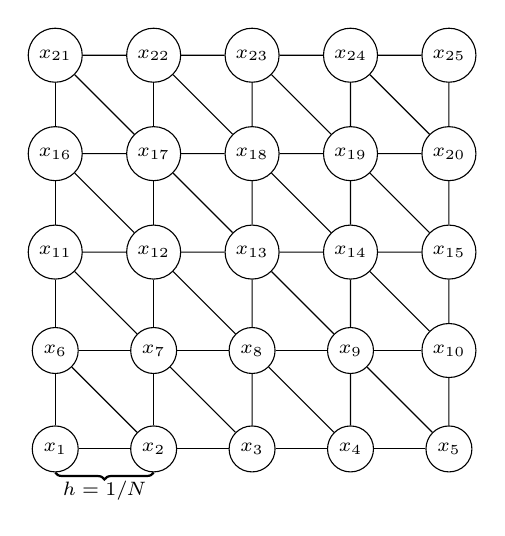
\begin{tikzpicture}[scale=5]

    \scriptsize
    % Place each of the nodes in the grid
    % First the boundary nodes

    % Place the nodes
    \foreach \x in {0,...,4}
        \foreach \y in {0,...,4}
    {
         \pgfmathtruncatemacro{\idx}{\y*5 + (\x + 1)}
         \node[circle,draw=black]
            (\x\y) at (0.25*\x,0.25*\y) {$x_{\idx}$};
    }

    % Next, the horizontal grid lines
    \foreach \y in {0,...,4}
       \foreach \x in {0,...,3}
    {
        \pgfmathtruncatemacro{\idx}{\x + 1}
        \draw (\x\y) -- (\idx\y);
    }

    % Now for the verticals
    \foreach \x in {0,...,4}
        \foreach \y in {0,...,3}
    {
        \pgfmathtruncatemacro{\idx}{\y + 1}
        \draw(\x\y) -- (\x\idx);
    }

    % Finally... the diagonals
    \foreach \y in {1,...,4}
        \foreach \x in {0,...,3}
    {
        \pgfmathtruncatemacro{\xidx}{\x + 1}
        \pgfmathtruncatemacro{\yidx}{\y - 1}
        \draw (\x\y) -- (\xidx\yidx);
    }

    % Bonus round, show the density of the grid
    \draw[thick,decoration={brace,mirror},decorate]
      (0,-0.06) -- (0.25, -0.06)
      node[pos=0.5,anchor=north]{$h=1/N$};
\end{tikzpicture}


\caption{Example triangulation of $D$ with $N = 4$}
\label{fig:two-d-discretisation}
\end{figure}

Using this triangulation we can now define suitable finite dimensional subspaces
of our test and trial spaces $V^h \subset V$, $W^h \subset W$:

\begin{align*}
    V^h &= \{v \in V: v \text{ is linear on } T_k,\ k \in \{1,\ldots,2N^2\},
                     v \text{ is continuous on } D\} \\
    W^h &= \{w \in W: w \text{ is linear on } T_k,\ k \in \{1,\ldots,2N^2\},
                     w \text{ is continuous on } D\}
\end{align*}

Then by choosing appropriate basis functions $\phi_i$ for the above subspaces
we will be able to approximate the solution as follows:

\begin{equation}
    u^h(\v{x}) = \sum_{j=0}^Mu_j\phi_j(\v{x})
\end{equation}

where $u_j$ will be the approximate value of the solution at the node $x_j$.
Similarly we can approximate $f(\v{x})$:

\begin{equation}
    f(x) \approx \sum_{j=0}^Mf_j\phi_j(\v{x})
\end{equation}

where $f_j = f(\v{x_j})$

As in the one dimensional case, an appropriate basis would be the `hat
functions' which we can define in terms of a reference function $\Phi(\v{x})$
defined with respect to an example domain around $(0,0)$.  Consider as in
Figure \ref{fig:reference-function-domain} the domain where the function has
support, then we can write $\Phi(\v{x})$ as follows:

\begin{equation}\label{eq:two-d-ref-basis-fn}
    \Phi(\v{x}) = \left\{\begin{array}{c c}
                    1 - x - y, & \text{ in } T_1 \\
                    1 - x,       & \text{ in } T_2 \\
                    1 + y,       & \text{ in } T_3 \\
                    1 + x + y,   & \text{ in } T_4 \\
                    1 + x,       & \text{ in } T_5 \\
                    1 - y,       & \text{ in } T_6 \\
                    0,           & \text{ otherwise}
                  \end{array}\right.
\end{equation}

where $\v{x} = (x, y)$. Then we can write each basis function $\phi_i$ in our
discretised domain as $\phi_i(\v{x}) = \Phi(\v{x} - \v{x_i})$

\begin{figure}
\centering
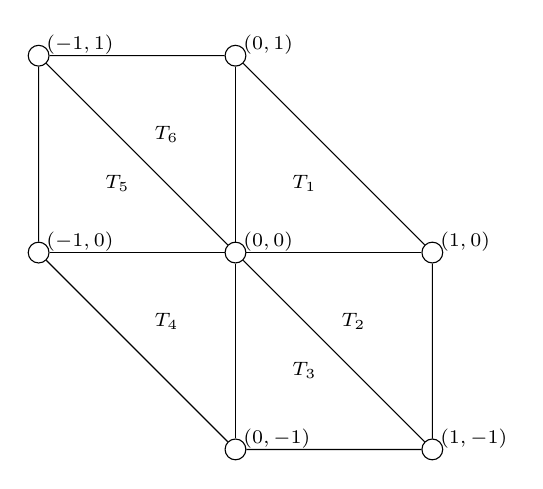
\begin{tikzpicture}[scale=2.5]
    \scriptsize

    % Place the nodes
    \node[circle,draw=black,label={[anchor=west]$(0,0)$}] (00)  at (0,0)  {};
    \node[circle,draw=black,label={[anchor=west]$(0,1)$}] (01)  at (0,1) {};
    \node[circle,draw=black,label={[anchor=west]$(1,0)$}] (10)  at (1,0)  {};
    \node[circle,draw=black,label={[anchor=west]$(-1,0)$}] (-10) at (-1,0) {};
    \node[circle,draw=black,label={[anchor=west]$(0,-1)$}] (0-1) at (0,-1) {};
    \node[circle,draw=black,label={[anchor=west]$(-1,1)$}] (-11) at (-1,1) {};
    \node[circle,draw=black,label={[anchor=west]$(1,-1)$}] (1-1) at (1,-1) {};

    % Draw the lines
    \draw (00) -- (01);
    \draw (00) -- (10);
    \draw (01) -- (10);
    \draw (00) -- (-10);
    \draw (00) -- (0-1);
    \draw (-11) -- (01);
    \draw (-11) -- (00);
    \draw (-11) -- (-10);
    \draw (-10) -- (0-1);
    \draw (0-1) -- (1-1);
    \draw (1-1) -- (10);
    \draw (00) -- (1-1);

    % Finally the T's
    \node (T1) at (0.35,0.35) {$T_1$};
    \node (T2) at (0.6, -0.35) {$T_2$};
    \node (T3) at (0.35, -0.6) {$T_3$};
    \node (T4) at (-0.35,-0.35) {$T_4$};
    \node (T5) at (-0.6, 0.35) {$T_5$};
    \node (T6) at (-0.35, 0.6) {$T_6$};

\end{tikzpicture}


\caption{The domain of the reference function $\Phi(\v{x})$}
\label{fig:reference-function-domain}
\end{figure}

Since the weak formulation \myref{eq:wk-twod-deterministic} has to hold forall
$v \in V$, in particular it has to hold for the basis functions
$\phi_i(\v{x})$, $i \in \{0,\ldots,M\}$ so by taking $v = \phi_i(\v{x})$ for
each $i \in \{0, \ldots, M\}$ and substituting our expansions for $u$ and $f$
we obtain:

\begin{align}
\begin{split}
    &a\int_{D}\nabla\phi_i(\v{x}) \cdot
                  \nabla\left(\sum_{j = 0}^Mu_j\phi_j(\v{x})\right)\, dD
    +\int_{D}\v{b}\cdot\phi_i(\v{x})\cdot
                  \nabla\left(\sum_{j = 0}^Mu_j\phi_j(\v{x})\right)\, dD \\
    &+c\int_{D}\phi_i(\v{x})
                    \left(\sum_{j = 0}^Mu_j\phi_j(\v{x})\right)\, dD =
    \int_{D}\left(\sum_{j = 0}^Mf_j\phi_j(\v{x})\right)
                 \phi_i(\v{x})\, dD
\end{split}
\end{align}

for each $i \in \{0, \ldots, M\}$ Then by the linearity of the integral and the
gradient operator this can be written as:

\begin{align}\label{eq:twod-deterministic-discrete}
  \begin{split}
    \sum_{j=0}^Mu_j
      \underbrace{\left(
         a\int_{D}\nabla\phi_i(\v{x})\cdot\nabla\phi_j(\v{x})\, dD
         + \v{b}\cdot\int_{D}\phi_i(\v{x})\cdot\nabla\phi_j(\v{x})\, dD
         +c\int_{D}\phi_i(\v{x})\phi_j(\v{x})\, dD
      \right)}_{:= A_{i,j}} = \\
    \sum_{j=0}^Mf_j
      \underbrace{\int_{D}\phi_i(\v{x})\phi_j(\v{x})}_{:= M_{i,j}}
  \end{split}
\end{align}

for $i \in \{1,\ldots,M\}$. This reduces the weak formulation
\myref{eq:wk-twod-deterministic} to a linear system $Au^h = Mf$ where as in the
one dimensional case $A$ is known as the stiffness matrix and $M$ is known as
the mass matrix. But due to the Dirichlet condition in
\myref{eq:two-d-deterministic} we already know the values of $u_j$ along the
boundary so the above reduces to:

\begin{equation}
    \sum_{j=1}^{(N-1)^2}A_{i,j}u_j =
    \sum_{j=0}^MM_{i,j}f_j
\end{equation}

for each $i \in \{1, \ldots, (N-1)^2\}$. Solving this system will give us an
approximation to the solution for \myref{eq:two-d-deterministic}.

\paragraph{Note:}

For convenience we can define the following \textit{bilinear form}:

\begin{equation}\label{eq:twod-deterministic-bilinear}
    \alpha(u,v) = a(\nabla u \cdot \nabla v) + u\v{b} \cdot \nabla v
                 + cuv
\end{equation}

which allows us to rewrite \myref{eq:twod-deterministic-discrete} as follows:

\begin{equation}
    \sum_{j = 0}^Mu_j\int_D\alpha(\phi_i,\phi_j)\, dD
        = \sum_{j = 0}^Mf_j\int_D\phi_i(\v{x})\phi_j(\v{x})\, dD
\end{equation}

\section{Constructing the Global System}

The last thing we need to do in order to implement the finite element method
for this problem is to determine the entries of the global mass and stiffness
matrices $M$ and $A$, respectively. Since we have discretised our domain into
many triangular elements, we can consider the contribution from each element
in turn and combine them into the global system.

Consider a triangular element $T$, comprised of the nodes $\v{k_1} = (0,0)$,
$\v{k_2} = (0,1)$, and $\v{k_3} = (1,0)$ with corresponding global basis functions
$\phi_{k_1}, \phi_{k_2}, \phi_{k_3}$. Now if we compare Figure
\ref{fig:twod-local-basis}, with Figure \ref{fig:reference-function-domain}
we see that the dashed lines denote the support of each of the basis functions
and the solid lines denote the subset of the domain which contains the triangular
element $T$.

Comparing further the two Figures we see that the triangular element $T$
corresponds to $T_1$ in the reference function for the basis function $\phi_{k1}$
and $T_5$ for $\phi_{k_2}$ and $T_3$ for $\phi_{k_3}$. This means locally in the
element $T_k$ we can define the following local basis functions:

\begin{align}\label{eq:twod-local-basis}
    \begin{split}
        \psi_1(x, y) = \Phi(\v{x} - \v{k_1})|_{T_1} &= 1 - x - y \\
        \psi_2(x, y) = \Phi(\v{x} - \v{k_2})|_{T_5} &= x \\
        \psi_3(x, y) = \Phi(\v{x} - \v{k_3})|_{T_3} &= y
    \end{split}
\end{align}

\begin{figure}
\centering
\begin{subfigure}[b]{0.30\textwidth}
    \centering
    \resizebox{\linewidth}{!}{\begin{tikzpicture}[scale=3]

    % Place the nodes of T_k
    \node[circle,draw=blue]  (k1) at (0,0) {\color{blue}$k_1$};
    \node (Tk) at (0.3, 0.3) {\color{blue}$T_k$};

    % Place the other nodes
    \node[circle,draw=black] (x0) at (-1,0) {};
    \node[circle,draw=black] (x1) at (0,-1) {};
    \node[circle,draw=black] (x2) at (-1,1) {};
    \node[circle,draw=black] (x3) at (1,-1) {};
    \node[circle,draw=black] (x4) at (1,0) {};
    \node[circle,draw=black] (x5) at (0,1) {};

    % Draw the triangle
    \draw[blue] (k1) -- (x5) -- (x4) --  (k1);
    \draw[dashed] (x5) -- (x2) -- (x0) -- (x1) -- (x3) -- (x4);
    \draw[dashed] (k1) -- (x0);
    \draw[dashed] (k1) -- (x1);
    \draw[dashed] (k1) -- (x2);
    \draw[dashed] (k1) -- (x3);

\end{tikzpicture}

}
\end{subfigure}
\begin{subfigure}[b]{0.30\textwidth}
    \centering
    \resizebox{\linewidth}{!}{\begin{tikzpicture}[scale=3]

    % Place the nodes of T_k
    \node[circle,draw=green]  (k2) at (0,0) {\color{green}$k_2$};
    \node (Tk) at (-0.6, 0.3) {\color{green}$T_k$};

    % Place the other nodes
    \node[circle,draw=black] (x0) at (-1,0) {};
    \node[circle,draw=black] (x1) at (0,-1) {};
    \node[circle,draw=black] (x2) at (-1,1) {};
    \node[circle,draw=black] (x3) at (1,-1) {};
    \node[circle,draw=black] (x4) at (1,0) {};
    \node[circle,draw=black] (x5) at (0,1) {};

    % Draw the triangle
    \draw[green] (k2) -- (x2) -- (x0) --  (k2);
    \draw[dashed] (x2) -- (x5) -- (x4) -- (x3) -- (x1) -- (x0);
    \draw[dashed] (k2) -- (x5);
    \draw[dashed] (k2) -- (x4);
    \draw[dashed] (k2) -- (x3);
    \draw[dashed] (k2) -- (x1);

\end{tikzpicture}

}
\end{subfigure}
\begin{subfigure}[b]{0.30\textwidth}
    \centering
    \resizebox{\linewidth}{!}{\begin{tikzpicture}[scale=3]

    % Place the nodes of T_k
    \node[circle,draw=red]  (k3) at (0,0) {\color{red}$k_3$};
    \node (Tk) at (0.3, -0.6) {\color{red}$T_k$};

    % Place the other nodes
    \node[circle,draw=black] (x0) at (-1,0) {};
    \node[circle,draw=black] (x1) at (0,-1) {};
    \node[circle,draw=black] (x2) at (-1,1) {};
    \node[circle,draw=black] (x3) at (1,-1) {};
    \node[circle,draw=black] (x4) at (1,0) {};
    \node[circle,draw=black] (x5) at (0,1) {};

    % Draw the triangle
    \draw[red] (k3) -- (x3) -- (x1) --  (k3);
    \draw[dashed] (x1) -- (x0) -- (x2) -- (x5) -- (x4) -- (x3);
    \draw[dashed] (k3) -- (x0);
    \draw[dashed] (k3) -- (x2);
    \draw[dashed] (k3) -- (x4);
    \draw[dashed] (k3) -- (x5);

\end{tikzpicture}

}
\end{subfigure}
\caption{Local contributions of the global basis functions
         $\phi_{k_1}, \phi_{k_2}, \phi_{k_3}$.}
\label{fig:twod-local-basis}
\end{figure}

This means that any $v \in V^h$ can locally in $T$ be written as:
\[
    v(\v{x}) = v(\v{k_1})\psi_1(\v{x}) + v(\v{k_2})\psi_2(\v{x}) + v(\v{k_3})\psi_3(\v{x})
\]

Furthermore, since we are using a uniform triangulation all of our triangles
are similar to this triangular element $T$ which we will now call the reference
triangle. Hence by introducing the mapping:

\begin{align*}
 \begin{array}{c c}
    \xi = \frac{x}{h} & \eta = \frac{y}{h}
 \end{array}
\end{align*}

we can map any triangular element $T_k$ in our discretisation onto the
reference triangle $T$ where $h$ represents the length of the sides of the
triangular element $T_k$. Hence we may write the local contribution of $T_k$ to
\myref{eq:twod-deterministic-discrete} as an integration around the reference
triangle $T$:

\begin{align}\label{eq:twod-deterministic-discrete-local}
    \begin{split}
    \sum_{r=1}^3\sum_{s=1}^3\underbrace{
      \left(
        ah^2\int_{T}\nabla\psi_r(\xi, \eta)\cdot\nabla\psi_s(\xi, \eta)\ d\xi d\eta
        + h^2\v{b} \cdot \int_{T}\psi_r(\xi,\eta)\cdot\nabla\psi_s(\xi,\eta)\ d\xi d\eta
        + ch^2\int_{T}\psi_r(\xi,\eta)\psi_s(\xi,\eta)\ d\xi d\eta
      \right)}_{A^{(k)}_{r,s}}u_s = \\
    \sum_{r=1}^3\sum_{s=1}^3\underbrace{\left(
        h^2\int_{T_k}\psi_r(\xi,\eta)\psi_s(\xi,\eta)\ d\xi d\eta
    \right)}_{M^{(k)}_{r,s}}f_s
    \end{split}
\end{align}

where $A^{(k)}$ and $M^{(k)}$ are the $3 \times 3$ local stiffness and mass
matrices respectively. Since evaluating their entries will involve derivatives
of the local basis functions we shall compute these now:

\begin{align}
    \begin{split}
        \nabla\psi_1(x, y) &= \left(\begin{array}{c} -1 \\ -1 \end{array}\right) \\
        \nabla\psi_2(x, y) &= \left(\begin{array}{c} 1 \\ 0 \end{array}\right) \\
        \nabla\psi_3(x, y) &= \left(\begin{array}{c} 0 \\ 1 \end{array}\right)
    \end{split}
\end{align}

\subsection{The Local Stiffness Matrix}:\label{sec:twod-deterministic-local-stiffness}

Similar to the one dimensional case, we now have an expression for the entries
of the local stiffness matrix, in terms of a number of integrals
\myref{eq:twod-deterministic-discrete-local} so we will only include a few
example cases and then present the results.

If we first consider the integral which gives the contribution from the
Laplacian:

\begin{equation*}
    ah^2\int_T\nabla\psi_r(\xi,\eta)\cdot\nabla\psi_s(\xi,\eta)\ d\xi d\eta =
    ah^2\int_T\psi_{r\xi}'\psi_{s\xi}' + \psi_{r\eta}'\psi_{s\eta}'\ d\xi d\eta
\end{equation*}

and if we take $r = 1$ and $s = 1$ then we get:

\begin{align*}
    ah^2\int_T(\psi_{i\xi}')^2 + (\psi_{1\eta}')^2\ d\xi d\eta
    &= ah^2\int_0^1\int_0^{1 - \eta}\frac{1}{h^2}((-1)^2 + (-1)^2)\ d\xi d\eta \\
    &= 2a\int_0^1\left[\xi\right]_0^{1 - \eta} \\
    &= 2a\left[\eta - \frac{\eta^2}{2}\right]_0^1 \\
    &= 2a\frac{1}{2} \\
    &= a
\end{align*}

Similarly let's consider the second integral corresponding to the gradient term,
in the case when $r = 1, s = 3$:

\begin{align*}
    h^2\int_T\psi_1(\xi,\eta)\v{b} \cdot \nabla\psi_3(\xi,\eta)\ d\xi d\eta
     &= h^2\int_0^1\int_0^{1-\eta}\frac{1}{h}(1 - \xi - \eta)
           \left(\begin{array}{c} b_1 \\b_2 \end{array}\right) \cdot
           \left(\begin{array}{c} 0 \\ 1 \end{array}\right)\ d\xi d\eta \\
     &= hb_2\int_0^1\int_0^{1-\eta} 1 - \xi - \eta \ d\xi d\eta \\
     &= hb_2\int_0^1\left[\xi - \frac{\xi^2}{2} - \eta\xi \right]_0^{1-\eta}\ d\eta \\
     &= hb_2\int_0^1(1 -\eta) - \eta(1-\eta) - \frac{(1 - \eta)^2}{2}\ d\eta \\
     &= hb_2\int_0^1\frac{1}{2} -\eta +\frac{\eta^2}{2}\ d\eta \\
     &= \left[\frac{\eta}{2} - \frac{\eta^2}{2} + \frac{\eta^3}{6}\right]_0^1 \\
     &= \frac{hb_2}{6}
\end{align*}

Now considering third integral, in the case where $r = 3, s = 2$:

\begin{align*}
    ch^2\int_T\psi_3(\xi,\eta)\psi_2(\xi,\eta)\ d\xi d\eta
    &= ch^2\int_0^1\int_0^{1-\eta}\xi\eta\ d\xi d\eta \\
    &= ch^2\int_0^1\left[\frac{\xi^2\eta}{2}\right]_0^{1-\eta}\ d\eta \\
    &= ch^2\int_0^1\frac{(1-\eta)^2\eta}{2}\ d\eta \\
    &= \frac{ch^2}{2}\left[\frac{\eta^2}{2} - \frac{2\eta^3}{3} - \frac{\eta^4}{4}\right]_0^1 \\
    &= \frac{ch^2}{24}
\end{align*}

Following a similar process for the rest of the entries gives us the following
form for the local stiffness matrix:

\begin{equation}\label{eq:twod-local-stiffness}
 A^{(k)} =
    \frac{a}{2}\left(\begin{array}{c c c}
         2 & -1 & -1 \\
        -1 &  1 &  0 \\
        -1 &  0 &  1
    \end{array}\right)
    + \frac{h}{12} \left(\begin{array}{c c c}
        -(b_1 + b_2) & 2b_1 & 2b_2 \\
        -(b_1 + b_2) & 2b_1  & 2b_2 \\
        -(b_1 + b_2) & 2b_1  & 2b_2
    \end{array}\right)
    + \frac{ch^2}{24}\left(\begin{array}{c c c}
         2 &  1 &  1 \\
         1 &  2 &  1 \\
         1 &  1 &  2
      \end{array}\right)
\end{equation}

where $a, c \in \mathbb{R}$ and $\v{b} = (b_1, b_2) \in \mathbb{R}^2$
correspond to the parameters which define the original equation
\myref{eq:two-d-deterministic} we considered.

\subsection{The Local Mass Matrix}\label{sec:twod-deterministic-local-mass}

Following the same procedure, we can also compute the entries of the local mass
matrix as defined in \myref{eq:twod-deterministic-discrete-local}, in fact the
entries of the mass matrix are the same as those in those in the third term of
the local stiffness matrix so we have already seen the case $r = 3, s = 2$ and
by the fact that the matrix is symmetric the case $r = 2, s = 3$. So let's
consider the case where $r = 1, s = 2$:

\begin{align*}
    h^2\int_T\psi_1(\xi,\eta)\psi_2(\xi,\eta)\ d\xi d\eta
    &=  h^2\int_0^1\int_0^{1-\eta}(1 - \xi -\eta)\xi\ d\xi d\eta \\
    &= h^2\int_0^1\left[\frac{\xi^2}{2} -\frac{\xi^3}{3}
                        -\frac{\xi^2\eta}{2}\right]_0^{1-\eta}\  d\eta \\
    &= h^2\int_0^1\frac{(1-\eta)^2}{2} - \frac{(1-\eta)^3}{3}- \frac{(1-\eta)^2\eta}{2}\ d\eta \\
    &= \frac{h^2}{6}\int_0^1(1- \eta)^3\ d\eta \\
    &= \frac{h^2}{6}\left[\eta -\frac{3\eta}{2} + \eta^3 - \frac{\eta^4}{4}\right]_0^1 \\
    &= \frac{h^2}{24}
\end{align*}

and by symmetry this is the same as the case $r = 2, s = 1$. Finally we can consider the case
$r = 1, s = 3$

\begin{align*}
    h_2\int_T\psi_1(\xi, \eta)\psi_3(\xi, \eta)\ d\xi d\eta
    &= h^2\int_0^1\int_0^{1-\eta}(1 - \xi - \eta)\eta\ d\xi d\eta \\
    &= h^2\int_0^1\left[\xi\eta - \frac{\xi^2\eta}{2} - \eta^2\xi\right]_0^{1-\eta}\ d\eta \\
    &= h^2\int_0^1(1-\eta)\eta - \frac{(1 - \eta)^2\eta}{2} - \eta^2(1 - \eta)\ d\eta \\
    &= \frac{h^2}{2}\int_0^1(1 - \eta)^2\eta \ d\eta \\
    &= \frac{h^2}{2}\left[\frac{\eta^2}{2} - \frac{2\eta^3}{2} + \frac{\eta^4}{4}\right]_0^1 \\
    &= \frac{h^2}{24}
\end{align*}

which again by symmetry will also give us the case where $r = 3, s = 1$. If we
follow the same procedure for the remaining diagonal elements we obtain the
following form for the local mass matrix:

\begin{equation}\label{eq:twod-local-mass}
    M^{(k)} =
    \frac{h^2}{24}\left(\begin{array}{c c c}
         2 &  1 &  1 \\
         1 &  2 &  1 \\
         1 &  1 &  2
      \end{array}\right)
\end{equation}

\subsection{Assembling the Global Stiffness Matrix}\label{sec:twod-global-stiffnes-assembly}

Now that we know the form of local stiffness matrix
\myref{eq:twod-local-stiffness} we can start to assemble the global stiffness
matrix. As in the one dimensional case, we need to take into account the
contributions each of the elements surrounding a node make to its value.

However the extra dimension does mean that there are a few more cases that we
have to consider. Firstly due to the boundary conditions on the problem only
the interior nodes are unknown - hence the fact that the global stiffness
matrix has dimension $(N - 1) \times (N - 1)$ it will be useful for us to
relabel the interior nodes to $X_k$, $k \in \{1, \ldots, (N-1)^2\}$ and let's
consider the $k$-th row of the global stiffness matrix:

\begin{align}
  \begin{split}
    A_{k,i} &= a\int_D\nabla\phi_k\cdot\nabla\phi_i\, dD
            + \v{b} \cdot \int_D\phi_k\cdot\nabla\phi_i\, dD
            + c\int_D\phi_k\phi_i\, dD \\
            &= \int_D\alpha(\phi_k,\phi_i)\, dD
  \end{split}
\end{align}

for each $i \in \{1,\ldots,(N-1)^2)\}$ and where we used the \textit{bilinear
form} we defined in \myref{eq:twod-deterministic-bilinear}. Looking at Figure
\ref{fig:twod-global-basis-contrib} we can see each of the values of $i$ where
the corresponding basis function $\phi_i$ has support in at least a subset of
the support of $\phi_k$. (Assuming that the node $X_k$ is on the interior of
the interior part of the domain).  This means the non zero entries in the
$k$-th row of $A$ are given by:

\begin{align}
  \begin{split}
      \int_D\alpha(\phi_k,\phi_k)\, dD
        &= 2\int_T\alpha(\psi_1,\psi_1)\, dT + 2\int_T\alpha(\psi_2,\psi_2)\, dT
         + 2\int_T\alpha(\psi_3,\psi_3)\, dT \\
      \int_D\alpha(\phi_k,\phi_{k+1})\, dD
          &= \int_T\alpha(\psi_1,\psi_2)\, dT + \int_T\alpha(\psi_2,\psi_1)\, dT \\
      \int_D\alpha(\phi_k,\phi_{k-1})\, dD
          &= \int_T\alpha(\psi_2,\psi_1)\, dT + \int_T\alpha(\psi_1,\psi_2)\, dT \\
      \int_D\alpha(\phi_k,\phi_{k+N})\, dD
          &= \int_T\alpha(\psi_3,\psi_1)\, dT + \int_T\alpha(\psi_1,\psi_3)\, dT \\
      \int_D\alpha(\phi_k,\phi_{k-N})\, dD
          &= \int_T\alpha(\psi_1,\psi_3)\, dT + \int_T\alpha(\psi_3,\psi_1)\, dT \\
      \int_D\alpha(\phi_k,\phi_{(k+1) - N})\, dD
          &= \int_T\alpha(\psi_2,\psi_3)\, dT + \int_T\alpha(\psi_3,\psi_2)\, dT \\
      \int_D\alpha(\phi_k,\phi_{(k-1) + N})\, dD
          &= \int_T\alpha(\psi_3,\psi_2)\, dT + \int_T\alpha(\psi_2,\psi_3)\, dT
  \end{split}
\end{align}

where again referring to Figure \ref{fig:twod-global-basis-contrib} you can see
where these basis functions share support and how they are rewritten locally in
that region with respect to the reference triangle $T$. Furthermore looking at
the definition of the local stiffness matrix \myref{eq:twod-local-stiffness}
and noting the fact that in the case of this problem and chosen discretisation
the local stiffness matrix takes the same form in each triangular element
$T_k$. Hence the non zero elements of the $k$-th row of $A$ are given by:

\begin{align}
  \begin{split}
    A_{k,k} &= 2\Ak{1}{1} + 2\Ak{2}{2} + 2\Ak{3}{3} \\
    A_{k,k+1} &= \Ak{1}{2} + \Ak{2}{1} \\
    A_{k,k-1} &= \Ak{2}{1} + \Ak{1}{2} \\
    A_{k,k+N} &= \Ak{3}{1} + \Ak{1}{3} \\
    A_{k,k-N} &= \Ak{1}{3} + \Ak{3}{1} \\
    A_{k,(k+1)-N} &= \Ak{2}{3} + \Ak{2}{3} \\
    A_{k,(k-1)+N} &= \Ak{3}{2} + \Ak{2}{3}
  \end{split}
\end{align}

\begin{figure}
    \centering
    \begin{subfigure}[b]{0.30\textwidth}
    \centering
    \resizebox{\linewidth}{!}{
        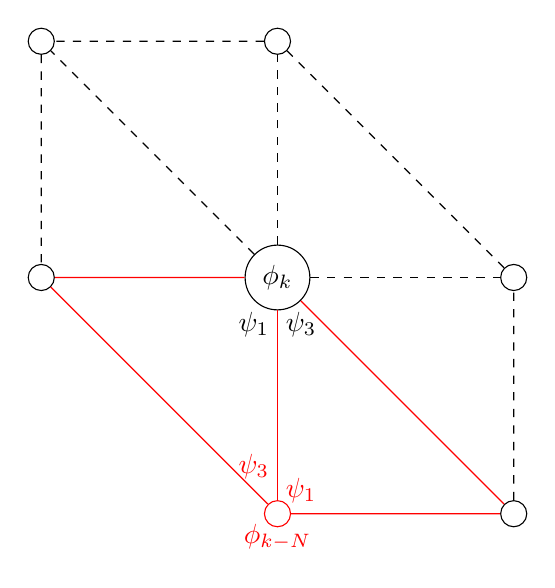
\begin{tikzpicture}[scale=3]
            % Place the center node
            \node[circle,draw=black] (k) at (0,0) {$\phi_k$};
            \node (p1) at (0.1, -0.2) {$\psi_3$};
            \node (p2) at (-0.1, -0.2) {$\psi_1$};
            \node (p2) at (-0.1, -0.8) {\color{red}$\psi_3$};
            \node (p1) at (0.1, -0.9) {\color{red}$\psi_1$};

            % Place the other nodes
            \node[circle,draw=black] (x0) at (-1,0) {};
            \node[circle,draw=red] (x1) at (0,-1) {};
            \node (k1) at (0, -1.1) {\color{red}$\phi_{k-N}$};
            \node[circle,draw=black] (x2) at (-1,1) {};
            \node[circle,draw=black] (x3) at (1,-1) {};
            \node[circle,draw=black] (x4) at (1,0) {};
            \node[circle,draw=black] (x5) at (0,1) {};

            % The lines!
            \draw[red] (k) -- (x0) -- (x1) -- (x3) -- (k);
            \draw[red] (k) -- (x1);
            \draw[dashed] (x3) -- (x4) -- (x5) -- (x2) -- (x0);
            \draw[dashed] (k) -- (x4);
            \draw[dashed] (k) -- (x5);
            \draw[dashed] (k) -- (x2);
        \end{tikzpicture}}
\end{subfigure}
\begin{subfigure}[b]{0.30\textwidth}
    \centering
    \resizebox{\linewidth}{!}{
        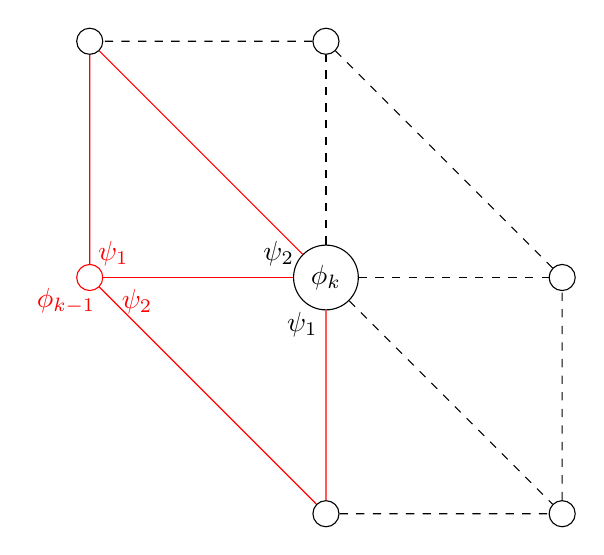
\begin{tikzpicture}[scale=3]
            % Place the center node
            \node[circle,draw=black] (k) at (0,0) {$\phi_k$};
            \node (p1) at (-0.2, 0.1) {$\psi_2$};
            \node (p2) at (-0.1, -0.2) {$\psi_1$};
            \node (p2) at (-0.8, -0.1) {\color{red}$\psi_2$};
            \node (p1) at (-0.9, 0.1) {\color{red}$\psi_1$};

            % Place the other nodes
            \node[circle,draw=red] (x0) at (-1,0) {};
            \node (k1) at (-1.1, -0.1) {\color{red}$\phi_{k-1}$};
            \node[circle,draw=black] (x1) at (0,-1) {};
            \node[circle,draw=black] (x2) at (-1,1) {};
            \node[circle,draw=black] (x3) at (1,-1) {};
            \node[circle,draw=black] (x4) at (1,0) {};
            \node[circle,draw=black] (x5) at (0,1) {};

            % The lines!
            \draw[red] (k) -- (x1) -- (x0) -- (x2) -- (k);
            \draw[red] (k) -- (x0);
            \draw[dashed] (x1) -- (x3) -- (x4) -- (x5) -- (x2);
            \draw[dashed] (k) -- (x5);
            \draw[dashed] (k) -- (x3);
            \draw[dashed] (k) -- (x4);
        \end{tikzpicture}}
\end{subfigure}
\begin{subfigure}[b]{0.30\textwidth}
    \centering
    \resizebox{\linewidth}{!}{
        \begin{tikzpicture}[scale=3]
            % Place the center node
            \node[circle,draw=black] (k) at (0,0) {$\phi_k$};
            \node (p1) at (-0.2, 0.1) {$\psi_2$};
            \node (p2) at (-0.1, 0.25) {$\psi_3$};
            \node (p2) at (-0.8, 0.9) {\color{red}$\psi_2$};
            \node (p1) at (-0.9, 0.8) {\color{red}$\psi_3$};

            % Place the other nodes
            \node[circle,draw=black] (x0) at (-1,0) {};
            \node[circle,draw=black] (x1) at (0,-1) {};
            \node[circle,draw=red] (x2) at (-1,1) {};
            \node (k1) at (-1, 1.15) {\color{red}$\phi_{(k-1) + N}$};
            \node[circle,draw=black] (x3) at (1,-1) {};
            \node[circle,draw=black] (x4) at (1,0) {};
            \node[circle,draw=black] (x5) at (0,1) {};

            % The lines!
            \draw[red] (k) -- (x5) -- (x2) -- (x0) -- (k);
            \draw[red] (k) -- (x2);
            \draw[dashed] (x0) -- (x1) -- (x3) -- (x4) -- (x5);
            \draw[dashed] (k) -- (x1);
            \draw[dashed] (k) -- (x3);
            \draw[dashed] (k) -- (x4);
        \end{tikzpicture}}
\end{subfigure}
\begin{subfigure}[b]{0.30\textwidth}
    \centering
    \resizebox{\linewidth}{!}{
        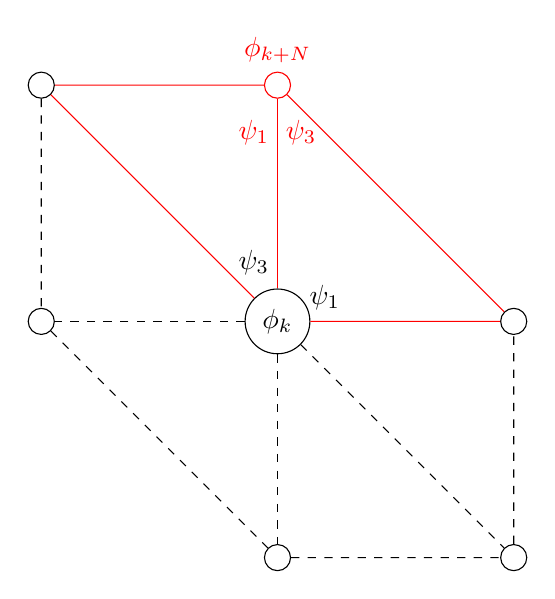
\begin{tikzpicture}[scale=3]
            % Place the center node
            \node[circle,draw=black] (k) at (0,0) {$\phi_k$};
            \node (p1) at (0.2, 0.1) {$\psi_1$};
            \node (p2) at (-0.1, 0.25) {$\psi_3$};
            \node (p2) at (0.1, 0.8) {\color{red}$\psi_3$};
            \node (p1) at (-0.1, 0.8) {\color{red}$\psi_1$};

            % Place the other nodes
            \node[circle,draw=black] (x0) at (-1,0) {};
            \node[circle,draw=black] (x1) at (0,-1) {};
            \node[circle,draw=black] (x2) at (-1,1) {};
            \node[circle,draw=black] (x3) at (1,-1) {};
            \node[circle,draw=black] (x4) at (1,0) {};
            \node[circle,draw=red] (x5) at (0,1) {};
            \node (k1) at (0, 1.15) {\color{red}$\phi_{k + N}$};

            % The lines!
            \draw[red] (k) -- (x4) -- (x5) -- (x2) -- (k);
            \draw[red] (k) -- (x5);
            \draw[dashed] (x2) -- (x0) -- (x1) -- (x3) -- (x4);
            \draw[dashed] (k) -- (x0);
            \draw[dashed] (k) -- (x1);
            \draw[dashed] (k) -- (x3);
        \end{tikzpicture}}
\end{subfigure}
\begin{subfigure}[b]{0.30\textwidth}
    \centering
    \resizebox{\linewidth}{!}{
        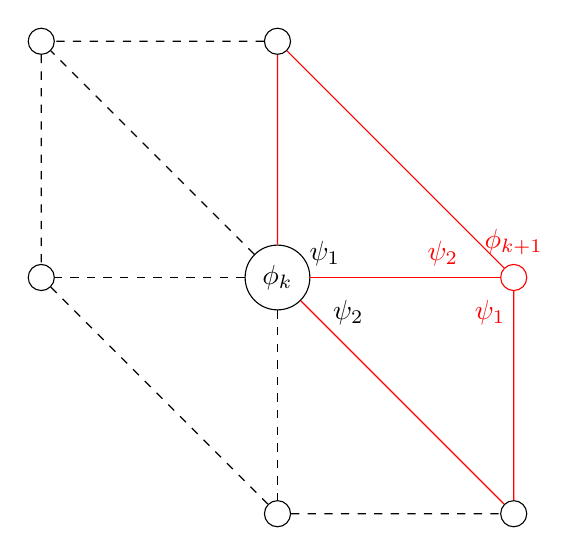
\begin{tikzpicture}[scale=3]
            % Place the center node
            \node[circle,draw=black] (k) at (0,0) {$\phi_k$};
            \node (p1) at (0.2, 0.1) {$\psi_1$};
            \node (p2) at (0.3, -0.15) {$\psi_2$};
            \node (p2) at (0.7, 0.1) {\color{red}$\psi_2$};
            \node (p1) at (0.9, -0.15) {\color{red}$\psi_1$};

            % Place the other nodes
            \node[circle,draw=black] (x0) at (-1,0) {};
            \node[circle,draw=black] (x1) at (0,-1) {};
            \node[circle,draw=black] (x2) at (-1,1) {};
            \node[circle,draw=black] (x3) at (1,-1) {};
            \node[circle,draw=red] (x4) at (1,0) {};
            \node (k1) at (1, 0.15) {\color{red}$\phi_{k+1}$};
            \node[circle,draw=black] (x5) at (0,1) {};

            % The lines!
            \draw[dashed] (x5) -- (x2) -- (x0) -- (x1) -- (x3);
            \draw[dashed] (k) -- (x2);
            \draw[dashed] (k) -- (x0);
            \draw[dashed] (k) -- (x1);
            \draw[red] (k) -- (x3) -- (x4) -- (x5) -- (k);
            \draw[red] (k) -- (x4);
        \end{tikzpicture}}
\end{subfigure}
\begin{subfigure}[b]{0.30\textwidth}
    \centering
    \resizebox{\linewidth}{!}{
        \begin{tikzpicture}[scale=3]
            % Place the center node
            \node[circle,draw=black] (k) at (0,0) {$\phi_k$};
            \node (p3) at (0.1, -0.3) {$\psi_3$};
            \node (p2) at (0.4, -0.15) {$\psi_2$};
            \node (p2) at (0.6, -0.9) {\color{red}$\psi_2$};
            \node (p3) at (0.9, -0.7) {\color{red}$\psi_3$};

            % Place the other nodes
            \node[circle,draw=black] (x0) at (-1,0) {};
            \node[circle,draw=black] (x1) at (0,-1) {};
            \node[circle,draw=black] (x2) at (-1,1) {};
            \node[circle,draw=red] (x3) at (1,-1) {};
            \node (k1) at (1, -1.1) {\color{red}$\phi_{(k + 1) - N}$};
            \node[circle,draw=black] (x4) at (1,0) {};
            \node[circle,draw=black] (x5) at (0,1) {};

            % The lines!
            \draw[dashed] (x4) -- (x5) -- (x2) -- (x0) -- (x1);
            \draw[dashed] (k) -- (x5);
            \draw[dashed] (k) -- (x2);
            \draw[dashed] (k) -- (x0);
            \draw[red] (k) -- (x1) -- (x3) -- (x4) -- (k);
            \draw[red] (k) -- (x3);
        \end{tikzpicture}}
\end{subfigure}
\begin{subfigure}[b]{0.30\textwidth}
    \centering
    \resizebox{\linewidth}{!}{
        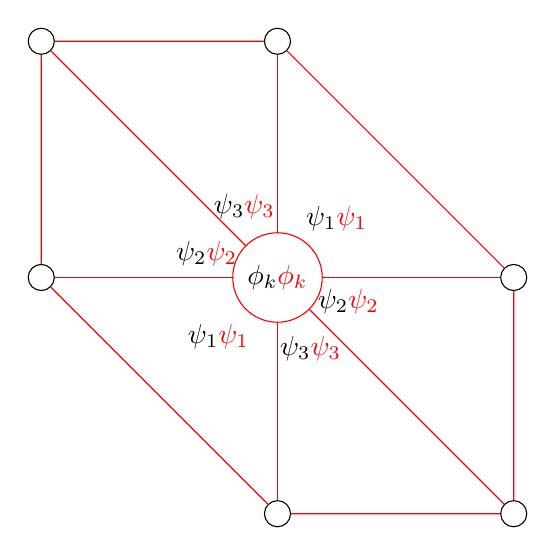
\begin{tikzpicture}[scale=3]
            % Place the center node
            \node[circle,draw=red] (k) at (0,0) {$\phi_k
                                                  \color{red}\phi_k$};
            \node (p1) at (0.14, -0.3){$\psi_3\color{red}\psi_3$};
            \node (p4) at (-0.14, 0.3) {$\psi_3\color{red}\psi_3$};
            \node (p2) at (-0.25, -0.25) {$\psi_1\color{red}\psi_1$};
            \node (p3) at (0.25, 0.25) {$\psi_1\color{red}\psi_1$};
            \node (p5) at (0.3, -0.1) {$\psi_2\color{red}\psi_2$};
            \node (p6) at (-0.3, 0.1) {$\psi_2\color{red}\psi_2$};

            % Place the other nodes
            \node[circle,draw=black] (x0) at (-1,0) {};
            \node[circle,draw=black] (x1) at (0,-1) {};
            \node[circle,draw=black] (x2) at (-1,1) {};
            \node[circle,draw=black] (x3) at (1,-1) {};
            \node[circle,draw=black] (x4) at (1,0) {};
            \node[circle,draw=black] (x5) at (0,1) {};

            % The lines!
            \draw[red] (x0) -- (x1) -- (x3) -- (x4) -- (x5) -- (x2) -- (x0);
            \draw[red] (k) -- (x0);
            \draw[red] (k) -- (x1);
            \draw[red] (k) -- (x2);
            \draw[red] (k) -- (x3);
            \draw[red] (k) -- (x4);
            \draw[red] (k) -- (x5);
        \end{tikzpicture}}
\end{subfigure}

    \caption{The contributions from the surrounding basis functions to the
        value at the node $x_k$}
    \label{fig:twod-global-basis-contrib}
\end{figure}

\paragraph{Note:}

The above only applies to nodes on the interior of the interior region - that
is nodes that are surrounded by other interior nodes. In the case of nodes on
the edge of this region their support intersects the support of nodes that are
known. In the case of these nodes the corresponding entry of the stiffness
matrix is set to zero and the value of the boundary node is taken to the right
hand side of the equation.

Let's consider an example, in the case where $N = 4$ - like in Figure
\ref{fig:two-d-discretisation} and take $a = 1, \v{b} = \v{0}, c = 0$
then the local stiffness matrix as given in
\myref{eq:twod-local-stiffness} will be given by:

\begin{equation}
    A^{(k)} = \frac{1}{2}\left[\begin{array}{c c c}
            2 & -1 & -1 \\ -1 & 1 & 0 \\ -1 & 0 & 1
    \end{array}\right]
\end{equation}

hence the non zero $i$-th entries of the $k$-th row will of the global
stiffness matrix are given by:

\begin{align}
  \begin{split}
    A_{k,k} &= \frac{2}{2}(2 + 1 + 1) = 4 \\
    A_{k,k+1} &= \frac{1}{2}(-1 -1) = -1 \\
    A_{k,k-1} &= \frac{1}{2}(-1 -1) = -1  \\
    A_{k,k+N} &= \frac{1}{2}(-1 -1) = -1 \\
    A_{k,k-N} &= \frac{1}{2}(-1 -1) = -1 \\
    A_{k,(k+1)-N} &= \frac{1}{2}(0 + 0) = 0 \\
    A_{k,(k-1)+N} &= \frac{1}{2}(0 + 0) = 0
  \end{split}
\end{align}

Therefore in this case the global stiffness matrix will be
$9 \times 9$ and take the following form:

\begin{equation}
    A = \left[\begin{array}{r r r r r r r r r}
        4 & -1 &  0 & -1 &  0 &  0 &  0 &  0 &  0 \\
       -1 &  4 & -1 &  0 & -1 &  0 &  0 &  0 &  0 \\
        0 & -1 &  4 &  0 &  0 & -1 &  0 &  0 &  0 \\
       -1 &  0 &  0 &  4 & -1 &  0 & -1 &  0 &  0 \\
        0 & -1 &  0 & -1 &  4 & -1 &  0 & -1 &  0 \\
        0 &  0 & -1 &  0 & -1 &  4 &  0 &  0 & -1 \\
        0 &  0 &  0 & -1 &  0 &  0 &  4 & -1 &  0 \\
        0 &  0 &  0 &  0 & -1 &  0 & -1 &  4 & -1 \\
        0 &  0 &  0 &  0 &  0 & -1 &  0 & -1 & 4
    \end{array}\right]
\end{equation}

\subsection{Assembling the Global Mass Matrix}

By following a similar argument to the case for the stiffness matrix and
considering Figure \ref{fig:two-d-discretisation} we find that the non zero
$i$-th entries of the $k$-th row are given by:

\begin{align}
  \begin{split}
    M_{k,k} &= 2\Mk{1}{1} + 2\Mk{2}{2} + 2\Mk{3}{3} \\
    M_{k,k+1} &= \Mk{1}{2} + \Mk{2}{1} \\
    M_{k,k-1} &= \Mk{2}{1} + \Mk{1}{2} \\
    M_{k,k+N} &= \Mk{3}{1} + \Mk{1}{3} \\
    M_{k,k-N} &= \Mk{1}{3} + \Mk{3}{1} \\
    M_{k,(k+1)-N} &= \Mk{2}{3} + \Mk{2}{3} \\
    M_{k,(k-1)+N} &= \Mk{3}{2} + \Mk{2}{3}
  \end{split}
\end{align}

So continuing the example we had in Section
\ref{sec:twod-global-stiffnes-assembly} with $N = 4 \rightarrow h = 1/4$ and
$a = 1, \v{b} = 0, c = 0$ then the local mass matrix as defined in
\myref{eq:twod-local-mass} is given by:

\begin{equation}\label{eq:twod-local-mass}
    M^{(k)} =
    \frac{1}{384}\left(\begin{array}{c c c}
         2 &  1 &  1 \\
         1 &  2 &  1 \\
         1 &  1 &  2
      \end{array}\right)
\end{equation}

hence the non zero $i$-th entries of the $k$-th row are given by:

\begin{align}
  \begin{split}
    M_{k,k} &= \frac{2}{384}(2 + 2 + 2) = \frac{12}{384}\\
    M_{k,k+1} &= \frac{1}{384}(1 + 1) = \frac{2}{384} \\
    M_{k,k-1} &= \frac{1}{384}(1 + 1) = \frac{2}{384} \\
    M_{k,k+N} &= \frac{1}{384}(1 + 1) = \frac{2}{384} \\
    M_{k,k-N} &= \frac{1}{384}(1 + 1) = \frac{2}{384} \\
    M_{k,(k+1)-N} &= \frac{1}{384}(1 + 1) = \frac{2}{384} \\
    M_{k,(k-1)+N} &= \frac{1}{384}(1 + 1) = \frac{2}{384}
  \end{split}
\end{align}

Therefore in this case the global mass matrix will be a $9 \times 25$ matrix of
the following form:

\begin{equation}
    M = \frac{1}{384}
        \left[\begin{array}{c c c c c c c c c c c c c c c c c c c c c c c c c}
    0 & 2 & 2 & 0 & 0 & 2 & 12 & 2 & 0 & 0 & 2 & 2 & 0 & 0 & 0 & 0 & 0 & 0 & 0 & 0 & 0 & 0 & 0 & 0 & 0 \\
    0 & 0 & 2 & 2 & 0 & 0 & 2 & 12 & 2 & 0 & 0 & 2 & 2 & 0 & 0 & 0 & 0 & 0 & 0 & 0 & 0 & 0 & 0 & 0 & 0 \\
    0 & 0 & 0 & 2 & 2 & 0 & 0 & 2 & 12 & 2 & 0 & 0 & 2 & 2 & 0 & 0 & 0 & 0 & 0 & 0 & 0 & 0 & 0 & 0 & 0 \\
    0 & 0 & 0 & 0 & 0 & 0 & 2 & 2 & 0 & 0 & 2 & 12 & 2 & 0 & 0 & 2 & 2 & 0 & 0 & 0 & 0 & 0 & 0 & 0 & 0 \\
    0 & 0 & 0 & 0 & 0 & 0 & 0 & 2 & 2 & 0 & 0 & 2 & 12 & 2 & 0 & 0 & 2 & 2 & 0 & 0 & 0 & 0 & 0 & 0 & 0 \\
    0 & 0 & 0 & 0 & 0 & 0 & 0 & 0 & 2 & 2 & 0 & 0 & 2 & 12 & 2 & 0 & 0 & 2 & 2 & 0 & 0 & 0 & 0 & 0 & 0 \\
    0 & 0 & 0 & 0 & 0 & 0 & 0 & 0 & 0 & 0 & 0 & 2 & 2 & 0 & 0 & 2 & 12 & 2 & 0 & 0 & 2 & 2 & 0 & 0 & 0 \\
    0 & 0 & 0 & 0 & 0 & 0 & 0 & 0 & 0 & 0 & 0 & 0 & 2 & 2 & 0 & 0 & 2 & 12 & 2 & 0 & 0 & 2 & 2 & 0 & 0 \\
    0 & 0 & 0 & 0 & 0 & 0 & 0 & 0 & 0 & 0 & 0 & 0 & 0 & 2 & 2 & 0 & 0 & 2 & 12 & 2 & 0 & 0 & 2 & 2 & 0
    \end{array}\right]
\end{equation}

\section{Example Problems and Results}

Just as in Chapter \ref{chap:oned-deterministic} to construct and solve these
linear systems we will have to make use of a computer. However in this case the
linear systems as discussed above \myref{eq:twod-deterministic-discrete} grow
on the order of $O(N^4)$ as opposed to $O(N^2)$ in the one dimensional case. In
order to handle the much greater computational complexity of these systems the
use of the Numpy linear algebra library has been replaced with the very similar
sparse section of the Scipy library \cite{scipy}.

The use of sparse matrices means memory usage and CPU time can be greatly
reduced allowing the us to handle these larger systems with relative ease. All
problems in this section have been solved using the code in Listing
\ref{code:twod-deterministic}. As with the one dimensional case the results
have been visualised with the Matplotlib library \cite{matplotlib}.

\begin{lstlisting}[language=Python,
                   caption={Setup code for the 2D Deterministic Finite Element
                            Method},
                   label={code:twod-deterministic}]
import numpy as np
from math import sin, cos, pi
import matplotlib.pyplot as plt
import seaborn as sns

sns.set_style('whitegrid')

from fem.twod_deterministic import solve_system, L2_error

a, b, c = # Coefficients are set depending on the problem

def u(x,y):
    # Exact solution is set depending on the problem

def f(x, y):
    # The RHS of the equation is set depending on the problem

def do_fem(f, a, b, c):

    NS = [4, 8, 16, 32, 64, 128, 256, 512]
    errors = []

    # For each mesh density
    for N in NS:

        # Solve the system
        xs, ys, U = solve_system(f, N, a, b, c)

        # Calculate the error
        errors.append(L2_error(u, U, N))

        # Plot one of the results
        if N == 64:
            fig, ax = plt.subplots(1)
            p = ax.pcolor(xs, ys, U, cmap='viridis')
            ax.set_xlabel(r"$x$", fontsize=18)
            ax.set_ylabel(r"$y$", fontsize=18)
            fig.colorbar(p)
            fig.savefig('twod-deterministic-approx.pdf')

    return (NS, errors), fig
\end{lstlisting}

For full details on the \incode{solve\_system} and \incode{L2\_error} functions
see Appendix \ref{app:twod-deterministic-code}.

Just as with the one dimensional case it's important that we verify the code
works as we intended so we in this case choose our solution to be
$u(\v{x}) = \sin{(\pi x)}\sin{(\pi y)}$ where $\v{x} = (x, y)$. By choosing
various values for $a, \v{b}$ and $c$ we can easily construct the right hand
side of the equation and having the solution in hand we can easily see the rate
of convergence of the finite element method.

Considering the following cases:
\begin{itemize}
    \item $a = 1, \v{b} = \v{0}, c = 0$ and
          $f(\v{x}) = 2\pi^2\sin{(\pi x)}\sin{(\pi y})$ \\
    \item $a = 1 \v{b} = \v{0}, c = 1$ and
          $f(\v{x}) = 2\pi^2\sin{(\pi x)}\sin{(\pi y)} +
                \sin{(\pi x)}\sin{(\pi y)}$ \\
    \item $a = 1, \v{b} = \v{0}, c = 0$ and
          $f(\v{x}) = 2\pi^2\sin{(\pi x)}\sin{(\pi y)} +
                10\sin{(\pi x)}\sin{(\pi y)}$
\end{itemize}

and recording the $L^2$ norm of the error at each value of $N$ we obtain the
plot seen in Figure \ref{fig:twod-deterministic-error}. In Figure
\ref{fig:twod-deterministic-exact-v-approx} we see the exact solution plotted
against one of our approximations in the case where $a = 1, \v{b} = \v{0}, c =
0$.

\begin{figure}
    \centering
    \begin{subfigure}[b]{0.75\textwidth}
        \centering
        \includegraphics[width=1\linewidth]{figures/twod-deterministic-exact.pdf}
    \end{subfigure}
    \begin{subfigure}[b]{0.75\textwidth}
        \centering
        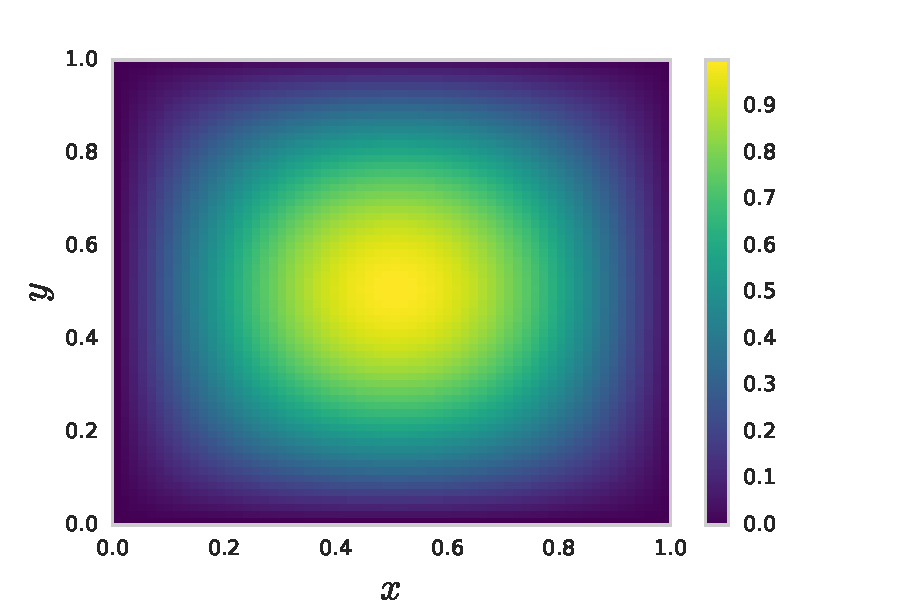
\includegraphics[width=1\linewidth]{figures/twod-deterministic-approx.pdf}
    \end{subfigure}
    \caption{Heatmap plots of the exact solution $u(\v{x})$ (top) against
             $u^h(\v{x})$ (bottom) with $N = 64$ in the case
             $a = 1, \v{b} = \v{0}, c = 0$}
    \label{fig:twod-deterministic-exact-v-approx}
\end{figure}

\begin{figure}
    \centering
    \includegraphics[width=0.75\linewidth]{figures/twod-deterministic-errors.pdf}
    \caption{Plot of $|| u - u^h ||_2$ for various values of  $N$}
    \label{fig:twod-deterministic-error}
\end{figure}


    \begin{appendices}
    	\chapter{One Dimensional Deterministic Calculations}

\section{Local Stiffness Matrix}

\subsection{The first integral}

These terms give the entries of the part of the local stiffness matrix multiplied 
by the parameter $a$ in \ref{eq:oned-deterministic-local-discrete}
In the case where $r = 2, s = 2$

\begin{align*}
  a\int_{x_k}^{x_{k+1}}\psi_{k,2}'(x)\psi_{k,2}'(x)\, dx 
    &= a\int_{x+k}^{x_{k+1}}\left(\frac{1}{x_{k+1} - x_k}\right)\, dx \\
    &= \frac{a}{h_k^2}\int_{x_k}^{x_{k+1}}1\, dx \\
    &= \frac{a}{h_k^2}(\underbrace{x_{k+1} - x_k}_{h_k}) \\
    &= \frac{a}{h_k}
\end{align*}

By symmetry we can see that the cases where $r = 1, s = 2$ and $r = 2, s = 1$ will
coincide:

\begin{align*}
	a\int_{x_k}^{x_{k+1}}\psi_{k, 1}'(x)\psi_{k, 2}'(x)\, dx
      &= a\int_{x_k}^{x_{k+1}}\left(\frac{-1}{x_{k+1} - x_k}\right)
                              \left(\frac{1}{x_{k+1} - x_k}\right)\, dx \\
      &= -\frac{a}{h_k^2}\int_{x_k}^{x_{k+1}}1\, dx \\
      &= -\frac{a}{h_k^2}(\underbrace{x_{k+1} - x_k}_{h_k}) \\
      &= -\frac{a}{h_k}
\end{align*}

\subsection{The second integral}

These terms correspond with the entries of the part of the local stiffness matrix
multiplied by the parameter $b$ in \ref{eq:oned-deterministic-local-discrete}

In the case where $r = 1, s = 1$:

\begin{align*}
	b\int_{x_k}^{x_{k+1}}\psi_{k,1}'(x)\psi_{k,1}(x)\, dx
      &= b\int_{x_k}^{x_{k+1}}\left(\frac{-1}{x_{k+1} - x_k}\right)
                              \left(\frac{x_{k+1} - x}{x_{k+1} - x_k}\right)\, dx \\
      &= -\frac{b}{h_k^2}\int_{x_k}^{x_{k+1}}(x_{k+1} - x)\, dx \\
      &= -\frac{b}{h_k^2}\left[x_{k+1}x - \frac{x^2}{2}\right]_{x_k}^{x_{k+1}} \\
      &= -\frac{b}{h_k^2}\left[\frac{x_k^2}{2} + x_{k+1}^2 -\frac{x_{k+1}^2}{2}
                               - x_kx_{k+1}\right] \\
      &= -\frac{b}{h_k^2}
            [\underbrace{x_{k+1}^2 - 2x_{k+1}x_k + x_k^2}_{(x_{k+1} - x_k)^2 = h_k^2}] \\
      &= -b
\end{align*}
        \chapter{One Dimensional Deterministic Code}\label{app:oned-deterministic-code}

Here is the code that implements the Finite Element Method as was described in
Chapter \ref{chap:oned-deterministic}

\lstinputlisting[language=Python]{src/fem/oned_deterministic.py}
        \chapter{Mesh Generation}

Here I outline the code which generates the mesh we need for various problems

\lstinputlisting[language=Python, firstline=120, lastline=123]{src/obj/generate.py}
\lstinputlisting[language=Python, firstline=125, lastline=133]{src/obj/generate.py}
\lstinputlisting[language=Python, firstline=135, lastline=138]{src/obj/generate.py}
\lstinputlisting[language=Python, firstline=140, lastline=148]{src/obj/generate.py}
\lstinputlisting[language=Python, firstline=150, lastline=153]{src/obj/generate.py}
\lstinputlisting[language=Python, firstline=155, lastline=163]{src/obj/generate.py}
\lstinputlisting[language=Python, firstline=165, lastline=168]{src/obj/generate.py}
\lstinputlisting[language=Python, firstline=170, lastline=178]{src/obj/generate.py}

        \chapter{Finite Element Method Implementation}

Here I outline the Python code which implements the finite
element method used in our numerical solutions.

\lstinputlisting[language=Python]{src/fem/system.py}
    \end{appendices}

    % The bibliography:
    \printbibliography
\end{document}
